% Рабочий черновик новой редакции главы 2.
% Текущий chapter_2.tex не изменен; этот файл предназначен для поэтапной замены после проверки.

\newpage
\begin{center}
  \textbf{\large ГЛАВА 2. Анализ клиентского взаимодействия ООО <<\_\_\_\_>> и проектирование клиентского цифрового контура}
\end{center}
\refstepcounter{chapter}
\addcontentsline{toc}{chapter}{ГЛАВА 2. Анализ клиентского взаимодействия ООО <<\_\_\_\_>> и проектирование клиентского цифрового контура}

\section{Характеристика объекта исследования и границы проектирования}

Вторая глава переводит теоретические положения первой главы в аналитико-проектную постановку для конкретного объекта исследования. Такой переход необходим потому, что информационная система в прикладной информатике рассматривается не как изолированная программа, а как совокупность программных, информационных, организационных и технологических средств, встроенных в деятельность пользователей и предприятия~\cite{utkin_baldin_2003,gost34003}. Следовательно, прежде чем задавать функции приложения, необходимо определить границы автоматизируемой деятельности, состав участников, состав данных и ограничения проектирования~\cite{kovalenko2014,gost34_601}.

Объектом исследования выступает ООО <<\_\_\_\_>>, действующее тематическое кафе-кофейня в стилистике Хогвартса. По результатам предпроектного обследования установлено, что заведение находится на раннем этапе работы: кафе уже открылось, прошла рекламная кампания у блогеров, появились первые посетители, при этом собственный устойчивый цифровой канал взаимодействия с гостями еще не сформирован. Данное состояние важно рассматривать не как зрелую операционную модель с накопленной статистикой, а как стартовую модель предприятия сферы HoReCa, в которой цифровой контур должен сначала обеспечить доступность информации, первичную фиксацию обращений и управляемость клиентских точек контакта~\cite{klientskiy_opyt_horeca,batsyna2020}.

Предметная специфика кафе определяется сочетанием трех признаков: общественное питание, событийный формат и тематический клиентский опыт. Для общественного питания цифровизация обычно затрагивает как производственно-учетные процессы, так и процессы клиентского обслуживания; однако исследователи ресторанной индустрии подчеркивают, что цифровая трансформация затрагивает не только внутреннюю автоматизацию, но и точки контакта с гостем до визита, во время визита и после него~\cite{alt2021,kandalenkova2023}. Поэтому проектируемая система в данной работе ограничивается клиентским цифровым контуром: меню, события, заявки на личные мероприятия, контакт с менеджером, пользовательские сценарии и геймифицированное вовлечение.

Такое ограничение не является упрощением объекта, поскольку оно соответствует фактической проблеме предприятия. На момент обследования у кафе отсутствуют сайт, собственный Telegram-канал и карточка на картах; до посещения гость получает информацию главным образом из рекламных материалов, причем эти материалы содержат только отдельные сведения о блюдах и не дают полноценного представления о мероприятиях. Если цифровое взаимодействие начинается только после физического прихода гостя, то предприятие теряет управляемость pre-visit этапа клиентского пути, который в исследованиях customer journey рассматривается как самостоятельная часть опыта, влияющая на последующее решение клиента~\cite{pantouvakis2022,rita2022,stickdorn2018}.

Организационная структура объекта также задает границы проектирования. В текущей модели выделяются владелец, управляющая, менеджер и сотрудники за стойкой; при этом заявки на мероприятия должны поступать менеджеру, а решение о дальнейшем контакте остается за сотрудником кафе. Следовательно, система не должна изображать полностью автоматическое бронирование как уже существующий процесс. Более корректная проектная постановка состоит в создании формы первичной заявки, где потенциальный клиент оставляет контактные данные и параметры события, после чего менеджер связывается с ним и согласует детали. Такая постановка согласуется с подходом трассируемости требований, согласно которому каждое требование должно выводиться из фактического источника потребности, роли пользователя или выявленного ограничения~\cite{mucha2024}.

\begin{table}[H]
\centering
\small
\caption{Характеристика объекта исследования и проектные следствия}
\label{tab:v2_object_characteristics}
\begin{tabularx}{\textwidth}{|>{\raggedright\arraybackslash}p{0.25\textwidth}|>{\raggedright\arraybackslash}p{0.37\textwidth}|>{\raggedright\arraybackslash}X|}
\hline
\textbf{Характеристика} & \textbf{Фактическое основание} & \textbf{Проектное следствие} \\ \hline
Ранний этап работы кафе & Кафе уже открыто, рекламная кампания проведена, поток посетителей только формируется & Эффект системы следует обосновывать через снижение информационного барьера и создание управляемого канала первичных обращений, а не через крупную экономию трудозатрат \\ \hline
Тематический формат & Ценность визита связана не только с блюдом, но и с атмосферой, событиями и образом участия гостя & Клиентский контур должен включать не только меню и контакты, но и геймифицированный сценарий, поддерживающий тематический опыт \\ \hline
Событийная модель развития & Планируются мастер-классы, личные мероприятия и дни рождения & Необходима форма заявки на мероприятие, публикация событий и структура данных для последующей обработки обращений менеджером \\ \hline
Отсутствие собственного цифрового канала & Нет сайта, собственного Telegram-канала и карточки на картах & Первым уровнем цифровизации становится публичная клиентская часть с актуальной информацией, контактами и понятным маршрутом обращения \\ \hline
Ручная фиксация обращений & Сведения о договоренностях находятся у менеджера в телефоне или передаются устно & Требуется структурировать минимальный набор данных заявки и обеспечить дальнейшую трассируемость статуса обращения \\ \hline
\end{tabularx}
\normalsize
\end{table}

Содержание таблицы~\ref{tab:v2_object_characteristics} показывает, что центральная проектная задача не сводится к созданию сайта-витрины. Если предприятие работает в условиях отсутствия собственного цифрового канала, то сайт или PWA становится точкой входа в более широкий клиентский цифровой контур: он связывает информацию о меню, информацию о событиях, заявку на личное мероприятие, контакт с менеджером и элементы вовлечения. В терминах сервис-дизайна такая система поддерживает не одну операцию, а последовательность touchpoints, из которых складывается клиентский опыт~\cite{stickdorn2018,pantouvakis2022}.

\begin{figure}[p]
    \centering
    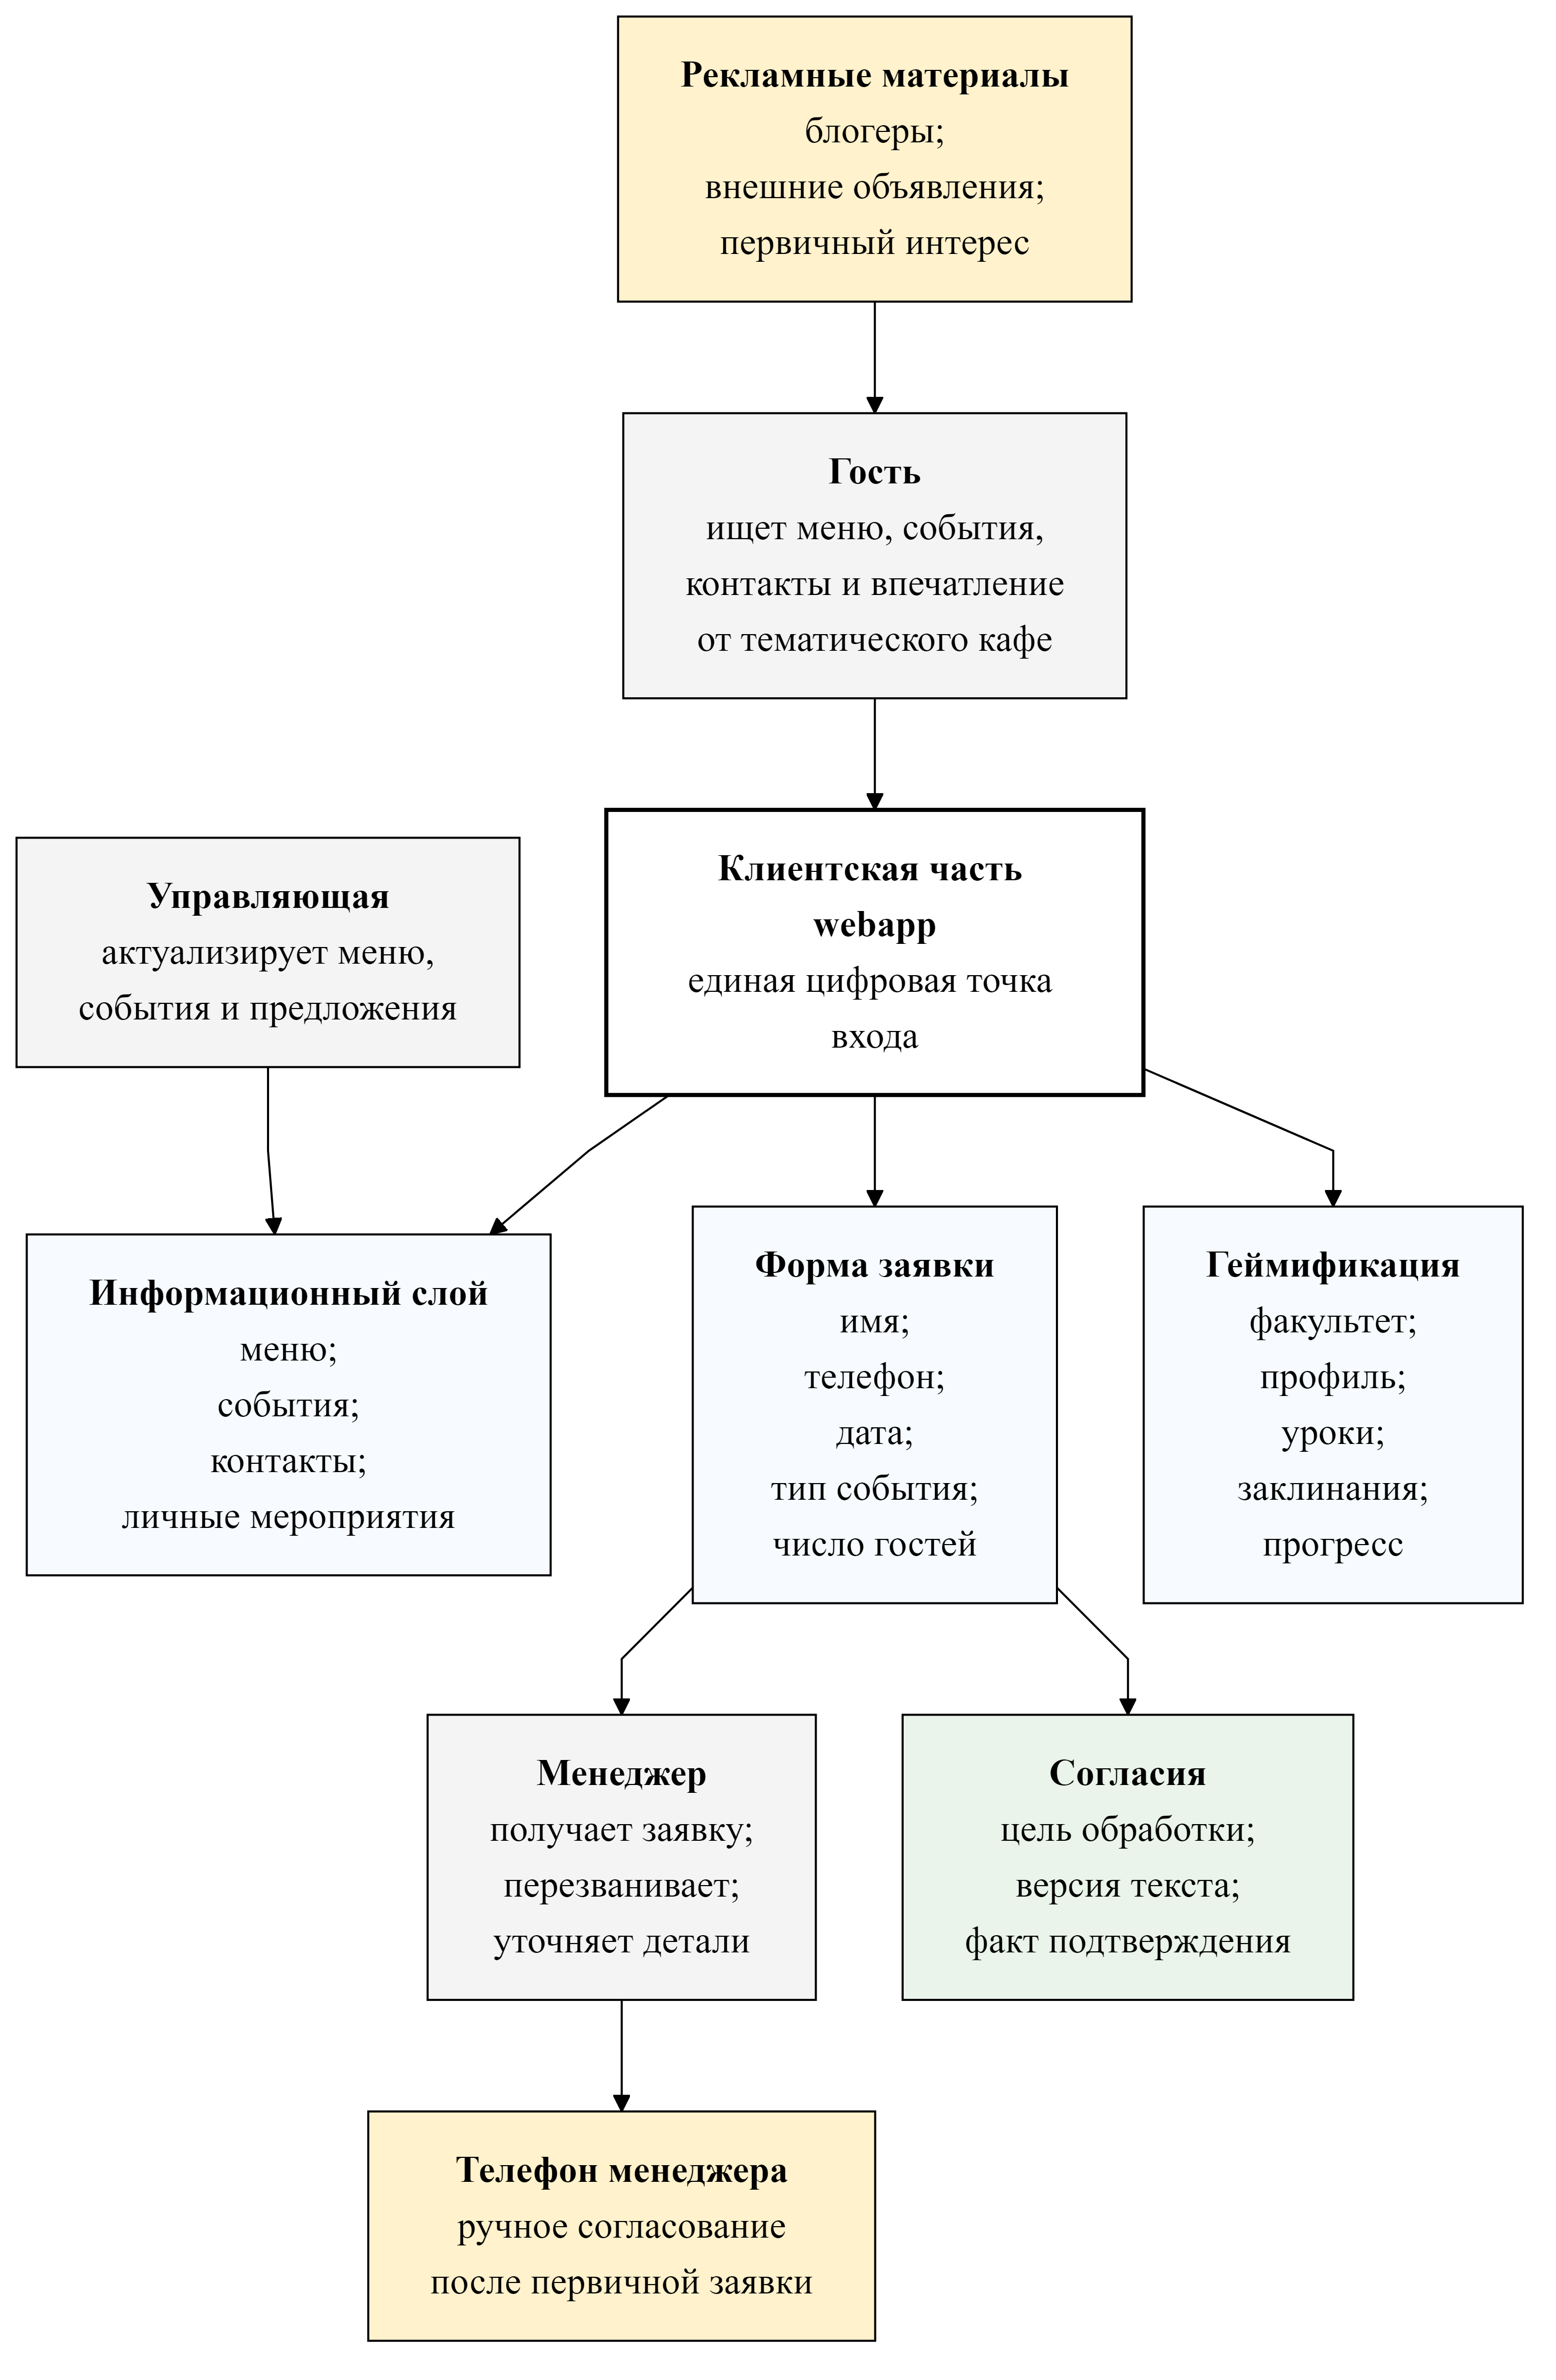
\includegraphics[width=0.98\textwidth,height=0.84\textheight,keepaspectratio]{figures/chapter2_v2_context.png}
    \caption{Контекст клиентского цифрового контура ООО <<\_\_\_\_>>}
    \label{fig:v2_context}
\end{figure}

Для настоящей работы принципиально важно отделить проектируемый клиентский контур от полной автоматизации предприятия общественного питания. Внутренние процессы кассы, склада, кухни, бухгалтерии и управленческого учета остаются за пределами второй главы, поскольку пользователь сформулировал задачу вокруг клиентской части, заявок и геймификации. Это соответствует рекомендациям по проектированию информационных систем: границы проекта должны определяться реальными целями автоматизации, доступными ресурсами, составом пользователей и ожидаемым способом внедрения~\cite{kovalenko2014,utkin_baldin_2003}. В дальнейшем расширении система может быть интегрирована с учетными или CRM-компонентами, но в текущей редакции ВКР такие компоненты должны рассматриваться как направление развития, а не как уже реализованная часть.

\section{Анализ текущего AS-IS клиентского взаимодействия}

Анализ AS-IS состояния нужен для того, чтобы проектные решения не возникали как произвольный набор функций. В работах по моделированию бизнес-процессов AS-IS модель описывает фактическое состояние процесса, а TO-BE модель строится как целевое состояние, устраняющее выявленные ограничения~\cite{ermilina2025,alieva2023}. Поэтому в данной главе сначала фиксируется реальный клиентский путь, затем из него выводятся проблемные зоны, требования и направления оптимизации.

Клиентское взаимодействие кафе удобно рассматривать через этапы пути гостя: до визита, во время визита и после визита. Такой способ анализа соответствует подходу customer journey, в котором сервис описывается не только внутренними действиями предприятия, но и последовательностью точек контакта, через которые проходит клиент~\cite{pantouvakis2022,stickdorn2018}. Для тематического кафе данный подход особенно важен, потому что ожидание гостя формируется до физического посещения: человек заранее оценивает блюда, атмосферу, возможность прийти на событие или организовать день рождения.

В текущем AS-IS состоянии pre-visit этап является наиболее слабым. До посещения потенциальный клиент узнает о кафе преимущественно из рекламных материалов, в которых присутствует информация только о некоторых блюдах и отсутствует полное описание мероприятий. Собственного сайта, Telegram-канала и карточки на картах на момент обследования нет, поэтому у гостя нет стабильного канала для самостоятельного уточнения меню, расписания, адресных данных, условий мастер-классов и возможностей личного мероприятия. С точки зрения исследований мобильных приложений питания, доступность фирменной информации на раннем этапе пути клиента влияет на поведенческое намерение использовать цифровой сервис и продолжить взаимодействие~\cite{rita2022}.

Физический этап взаимодействия сейчас компенсирует часть цифрового дефицита. В самом заведении есть буклет с меню, а сведения о возможности частного мероприятия можно получить через личное присутствие или контакт с менеджером. Однако такое решение не устраняет проблему pre-visit этапа, поскольку гость должен сначала прийти в кафе или получить номер менеджера из внешнего рекламного контекста. Следовательно, информация о ключевой коммерческой услуге, личных мероприятиях и днях рождения, не встроена в управляемый клиентский путь.

Процесс заявки на мероприятие в текущем виде также остается слабо структурированным. По фактическим сведениям, забронировать мероприятие можно по номеру телефона менеджера, а данные о договоренностях находятся у менеджера в телефоне. В такой модели отсутствует единая форма первичного обращения, единый состав полей, единый статус обработки и единая история изменений. В терминах информационных систем это означает, что данные возникают, но не преобразуются в управляемый информационный ресурс предприятия~\cite{utkin_baldin_2003,gost34003}.

Обратная связь в AS-IS модели фиксируется устно и не обрабатывается системно. Это ограничение важно не потому, что у молодого кафе уже должна существовать развитая аналитика, а потому, что без структурированной обратной связи предприятие не создает базу для последующего улучшения сервиса, персонализации предложений и оценки реакции на события. В исследованиях клиентского вовлечения обратная связь, участие клиента и повторные действия рассматриваются как элементы более широкого взаимодействия, влияющего на будущую ценность отношений между клиентом и организацией~\cite{pansari2017,behnam2021,chathoth2016}.

\begin{table}[H]
\centering
\small
\caption{AS-IS клиентский путь кафе}
\label{tab:v2_asis_customer_journey}
\begin{tabularx}{\textwidth}{|>{\raggedright\arraybackslash}p{0.18\textwidth}|>{\raggedright\arraybackslash}p{0.52\textwidth}|>{\raggedright\arraybackslash}X|}
\hline
\textbf{Этап} & \textbf{Текущий контакт и решение клиента} & \textbf{Ограничение AS-IS} \\ \hline
До визита & Контакт: рекламные материалы у блогеров и иные рекламные сообщения. Решение: первичное впечатление о концепции, отдельных блюдах и возможности посещения. & Нет единого источника полной информации о меню, событиях, контактах и возможностях личного мероприятия \\ \hline
Перед решением о событии & Контакт: номер телефона менеджера, если клиент смог его получить. Решение: желание узнать условия дня рождения, мастер-класса или частного мероприятия. & Канал обращения не очевиден для клиента, а состав первичной заявки заранее не нормирован \\ \hline
Во время визита & Контакт: буклет с меню, устные разъяснения сотрудников. Решение: выбор блюд, уточнение формата кафе, вопросы о мероприятиях. & Информация доступна уже после прихода, поэтому не работает как инструмент предварительного выбора \\ \hline
После визита & Контакт: устная обратная связь и возможное повторное личное обращение. Решение: оценка опыта, интерес к повторному визиту или событию. & Нет системной фиксации обратной связи и связи отзыва с конкретным клиентским сценарием \\ \hline
\end{tabularx}
\normalsize
\end{table}

Из таблицы~\ref{tab:v2_asis_customer_journey} следует, что текущий процесс нельзя описывать как неэффективный из-за большого числа потерянных заявок, поскольку таких количественных данных пока нет. Более строгий аналитический вывод состоит в другом: предприятие уже формирует рыночный интерес через рекламу, но не имеет собственного цифрового механизма, который превращает этот интерес в структурированное обращение. Поэтому дефицит AS-IS состояния относится не к скорости обработки большого потока, а к отсутствию устойчивой связки между вниманием потенциального клиента, информацией о предложении и первичным контактом с менеджером.

Отдельно следует рассмотреть роль геймификации в AS-IS состоянии. Физическая концепция кафе уже задает тематический контекст, однако до внедрения клиентской части этот контекст почти не продолжается в цифровой среде. На уровне существующего webapp уже предусмотрены игровые сущности: факультеты, пользовательский профиль, уровни мастерства, заклинания, уроки и элементы прогресса. С научной точки зрения это не является заменой основной услуги, потому что геймификация определяется как применение элементов игрового дизайна в неигровом контексте~\cite{deterding2011}. Следовательно, в проектируемой системе она должна рассматриваться как способ усиления клиентского опыта и удержания внимания вокруг тематического кафе, а не как самостоятельная игра, оторванная от бизнес-процесса.

\begin{table}[H]
\centering
\small
\caption{AS-IS состояние по ключевым информационным объектам}
\label{tab:v2_asis_information_objects}
\begin{tabularx}{\textwidth}{|>{\raggedright\arraybackslash}p{0.24\textwidth}|>{\raggedright\arraybackslash}p{0.34\textwidth}|>{\raggedright\arraybackslash}X|}
\hline
\textbf{Информационный объект} & \textbf{Текущее состояние} & \textbf{Последствие для проектирования} \\ \hline
Меню & Полное меню доступно в заведении в виде буклета, до визита клиент видит только отдельные блюда из рекламы & Требуется цифровое меню, которое снижает неопределенность до посещения и может обновляться без печатного цикла \\ \hline
События и мастер-классы & Мастер-классы планируются, но управляемого публичного расписания пока нет & Нужен раздел событий с возможностью последующего подключения записи или заявки \\ \hline
Личные мероприятия и дни рождения & Это значимое направление развития, но канал первичного обращения не встроен в публичный цифровой путь & Нужна форма заявки с минимальным набором полей и возможностью прямого звонка менеджеру \\ \hline
Контактные данные клиента & Передаются менеджеру вручную или устно & Необходимы согласие на обработку персональных данных, цель обработки и ограничение состава данных~\cite{fz152,moric2024} \\ \hline
Обратная связь & Существует в устной форме и не образует структурированной истории & Следует заложить возможность последующей фиксации отзывов, реакций и пользовательских действий \\ \hline
Тематический прогресс & В физическом AS-IS процессе не является управляемым цифровым объектом & Геймификация может стать отдельным цифровым слоем, связанным с вовлечением и повторными действиями \\ \hline
\end{tabularx}
\normalsize
\end{table}

Таблица~\ref{tab:v2_asis_information_objects} показывает, что исходная проблема находится на стыке информации, сервиса и маркетингового взаимодействия. Кафе уже обладает содержанием, которое можно предъявить клиенту: меню, тематическая атмосфера, будущие мастер-классы, возможность личных мероприятий. Однако это содержание пока не собрано в единый цифровой интерфейс, поэтому клиентский путь зависит от рекламных фрагментов, личного присутствия и индивидуального контакта с менеджером. В терминах service design такая ситуация означает разрыв между touchpoints: отдельные контакты существуют, но не образуют согласованную последовательность опыта~\cite{stickdorn2018,pantouvakis2022}.

\begin{figure}[p]
    \centering
    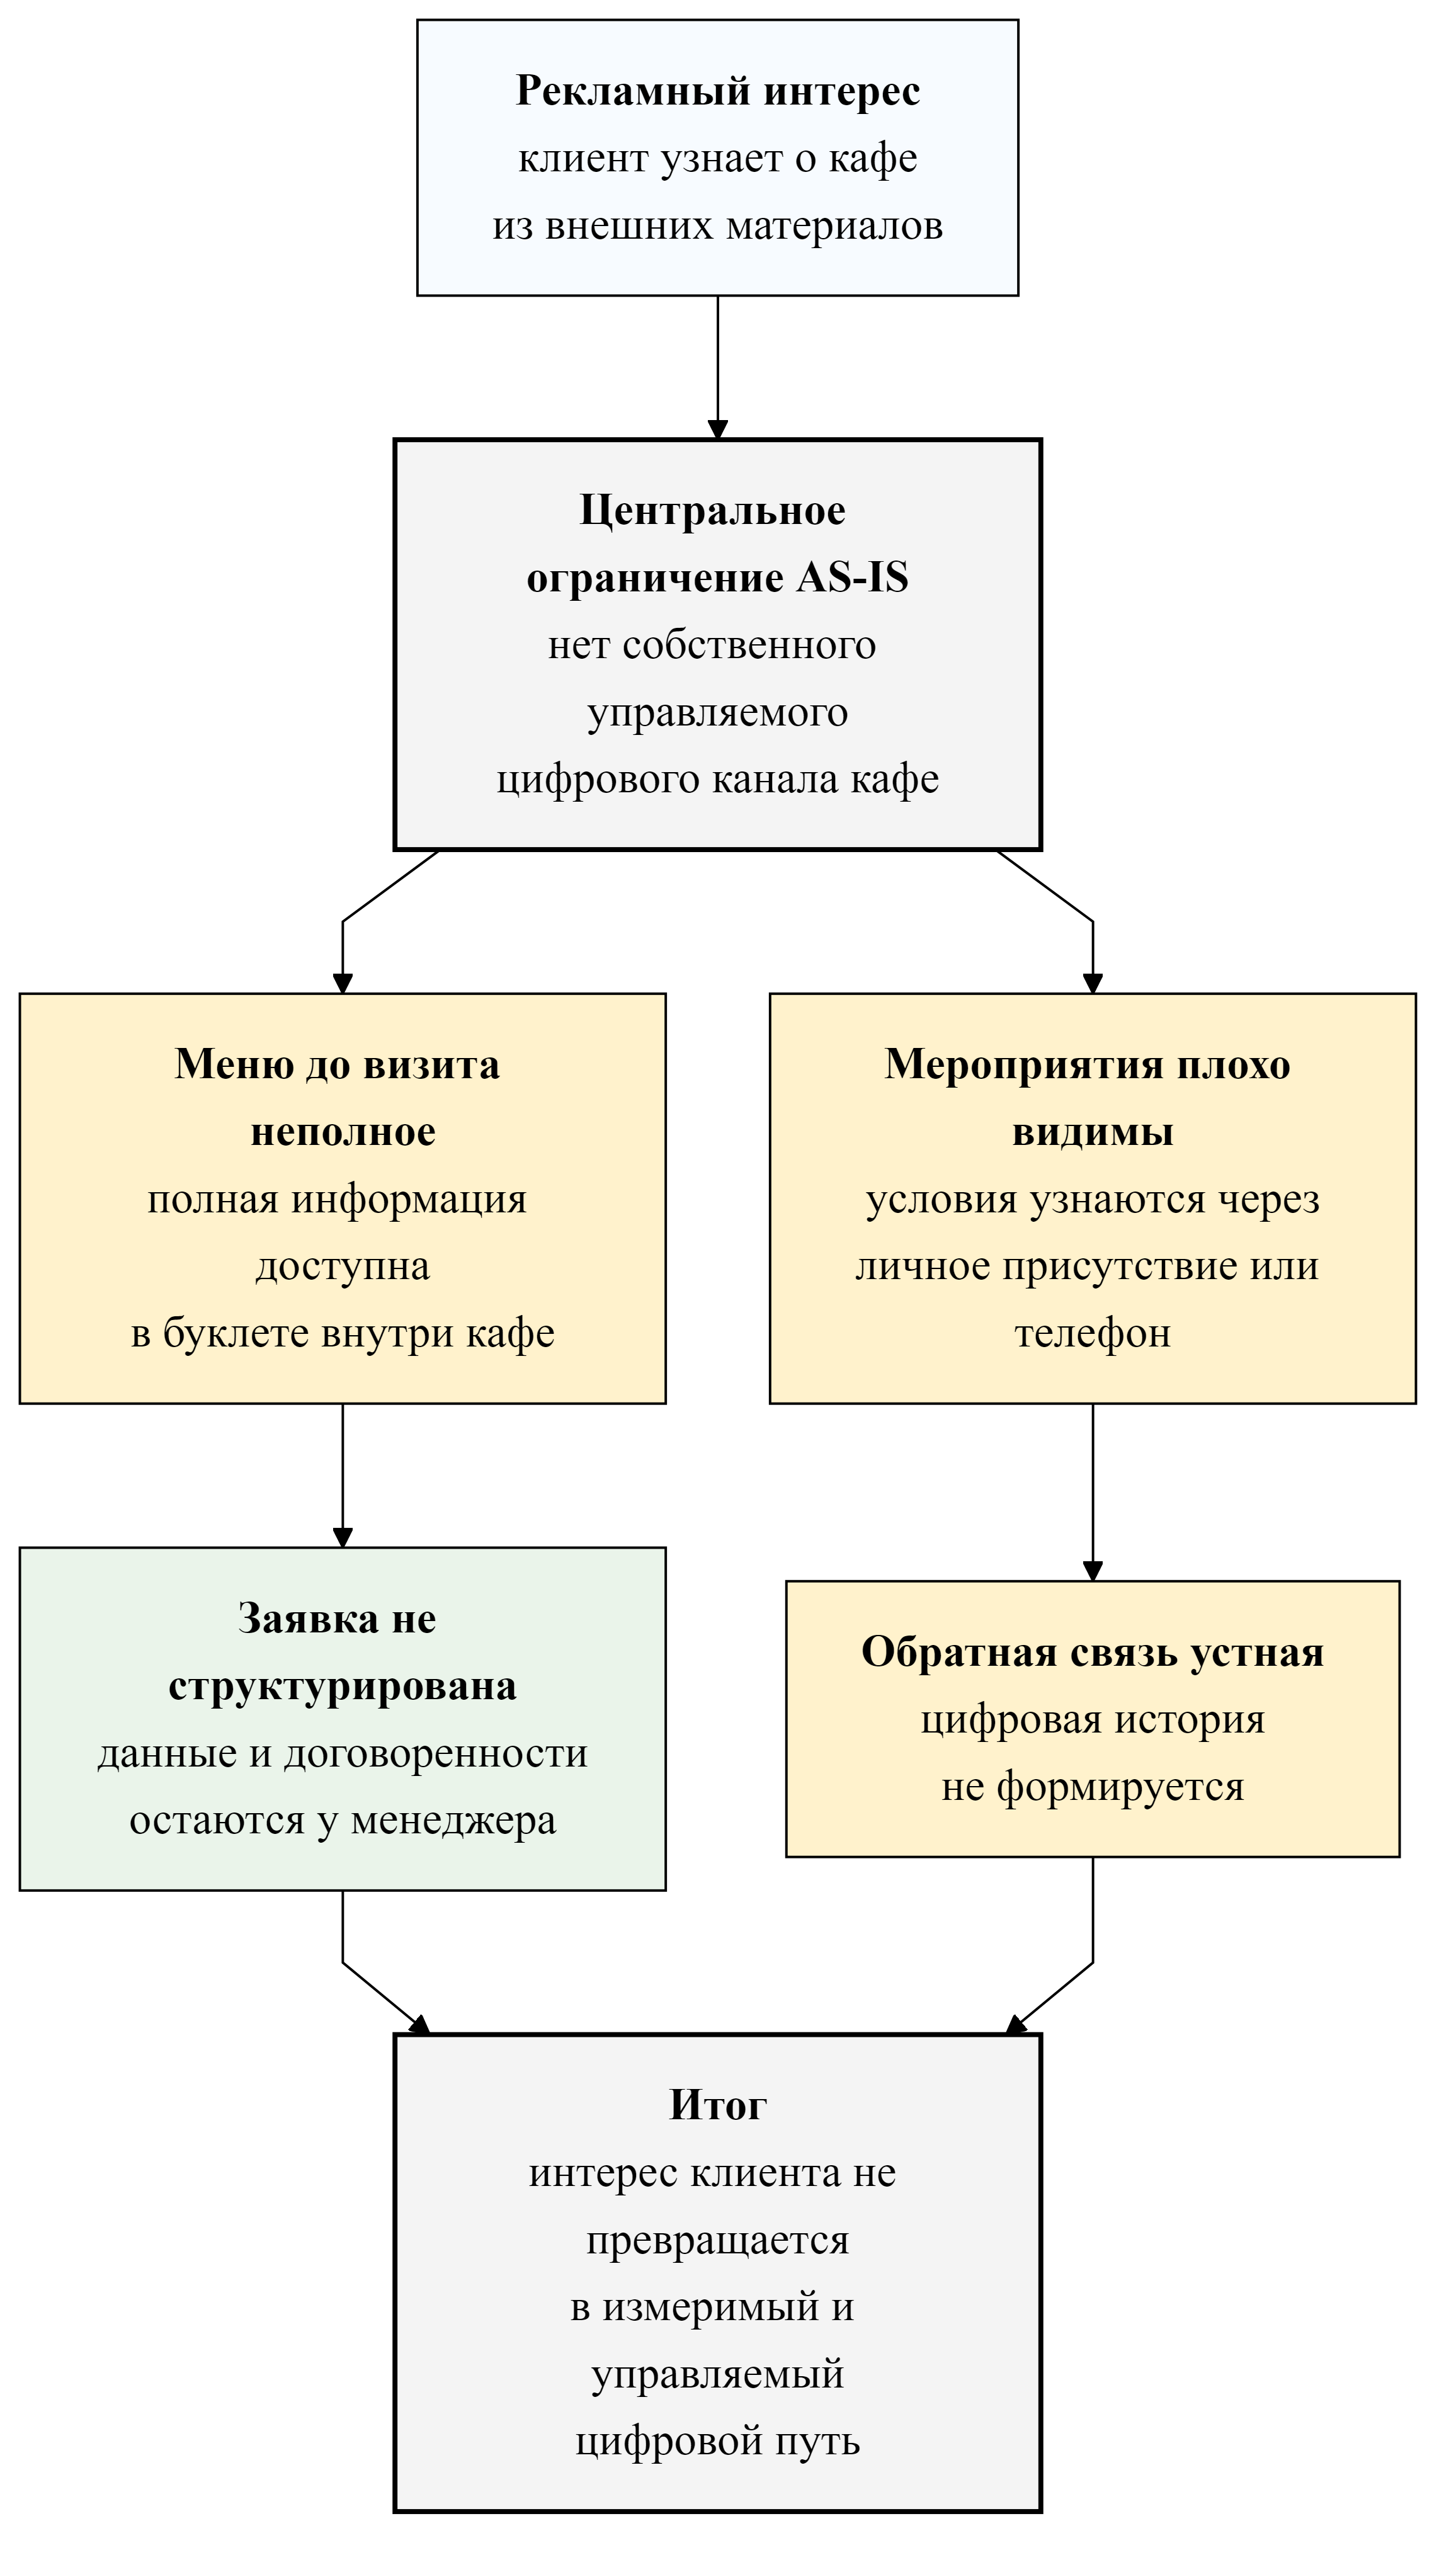
\includegraphics[width=0.98\textwidth,height=0.82\textheight,keepaspectratio]{figures/chapter2_v2_asis_journey.png}
    \caption{AS-IS клиентский путь до внедрения собственного цифрового канала}
    \label{fig:v2_asis_journey}
\end{figure}

\section{Выявление проблемных участков и причин ограничений}

Проблемные участки AS-IS процесса следует формулировать осторожно, потому что кафе находится на раннем этапе работы и пока не имеет большого массива заявок, статистики конверсии или измеренного времени обработки обращений. Поэтому в данной главе нецелесообразно доказывать значительную экономию времени менеджера или резкое снижение операционных затрат. Более корректный вывод состоит в том, что проектируемая система создает необходимые условия для управляемого роста клиентского взаимодействия: снижает информационный барьер до визита, структурирует первичные обращения, задает основу клиентской базы и переносит тематический опыт в цифровой канал~\cite{alt2021,batsyna2020,klientskiy_opyt_horeca}.

Методологически выявленные проблемы должны быть связаны с будущими требованиями. В исследованиях redesign подчеркивается, что проектирование TO-BE процесса должно опираться на выявленные performance issues, критерии оценки и анализ применимости решения до внедрения~\cite{maruster2009,tsakalidis2024}. В работах по трассируемости требований также показано, что связь между источником потребности и требованием помогает объяснить, почему функция появилась в системе и какой роли она служит~\cite{mucha2024}. Поэтому далее каждая проблема формулируется не как общее пожелание, а как связка ``факт AS-IS -> причина -> проектное требование''.

Первый проблемный участок связан с отсутствием собственного цифрового канала. Реклама у блогеров привлекает внимание, но рекламное сообщение не предназначено для постоянного хранения актуального меню, расписания событий, адресной информации, условий личных мероприятий и контактной формы. Следовательно, после возникновения интереса клиент не получает управляемую точку продолжения взаимодействия. Для молодого предприятия это особенно критично, потому что ранний интерес нужно переводить в повторяемый процесс обращения, а не оставлять в виде разрозненных сообщений.

Второй проблемный участок связан с неполной доступностью информации до визита. Если полное меню доступно только внутри заведения, а сведения о мероприятиях и частных событиях не опубликованы в структурированном виде, то клиент принимает решение на основании неполной информации. В исследованиях мобильных сервисов питания фирменная информация рассматривается как фактор клиентского пути на ранней стадии выбора~\cite{rita2022}. Следовательно, цифровое меню и раздел событий должны рассматриваться не как декоративные страницы, а как элементы снижения неопределенности перед визитом.

Третий проблемный участок относится к заявкам на личные мероприятия. Существующая модель, где обращение проходит через телефон менеджера и фиксируется в личном устройстве, приемлема на старте при малом числе обращений, но плохо масштабируется как организационная практика. Причина состоит не только в возможной потере сообщения, а в отсутствии нормированной структуры данных: цель мероприятия, дата, количество гостей, контактное лицо, комментарий, статус обработки и история контакта не образуют единого объекта. Для информационной системы это означает отсутствие устойчивой сущности ``заявка'', из которой далее можно построить обработку, аналитику и контроль исполнения~\cite{gost34003,utkin_baldin_2003}.

Четвертый проблемный участок связан с обратной связью и повторным взаимодействием. Устные отзывы помогают сотрудникам понимать реакцию гостей, но не создают цифрового следа, который можно связать с событием, меню, геймифицированной активностью или повторным интересом. Исследования customer engagement показывают, что вовлечение включает не только транзакцию, но и поведенческие, эмоциональные и когнитивные формы участия клиента~\cite{pansari2017,behnam2021}. Поэтому будущая система должна закладывать основу для таких действий, даже если полноценная аналитика будет развиваться позже.

Пятый проблемный участок является специфичным именно для тематического кафе. Физическая атмосфера в стилистике Хогвартса формирует ожидание игрового или ролевого взаимодействия, однако без цифрового продолжения этот опыт заканчивается в момент рекламного просмотра или физического визита. Геймификация позволяет связать тематический образ кафе с действиями пользователя в цифровой среде: выбор факультета, накопление прогресса, прохождение уроков, открытие заклинаний, участие в событиях и возвращение к контенту. Поскольку геймификация в научной литературе определяется как использование элементов игрового дизайна в неигровом контексте, она в данной работе должна быть обоснована через задачи вовлечения, удержания внимания и усиления клиентского опыта~\cite{deterding2011,chathoth2016,xu2017,buil2024}.

\begin{table}[H]
\centering
\small
\caption{Проблемные участки AS-IS процесса и выводимые требования}
\label{tab:v2_problems_requirements}
\begin{tabularx}{\textwidth}{|>{\raggedright\arraybackslash}p{0.24\textwidth}|>{\raggedright\arraybackslash}p{0.45\textwidth}|>{\raggedright\arraybackslash}X|}
\hline
\textbf{Проблемный участок} & \textbf{Причина ограничения и требование} & \textbf{Основание} \\ \hline
Нет собственного цифрового канала & Причина: рекламные материалы не являются постоянной управляемой точкой контакта. Требование: создать клиентскую веб-часть с меню, событиями, контактами и маршрутами обращения. & Customer journey и управление touchpoints~\cite{stickdorn2018,pantouvakis2022} \\ \hline
Неполная информация до визита & Причина: меню и условия событий не опубликованы в едином публичном источнике. Требование: разместить цифровое меню, раздел событий и описание форматов личных мероприятий. & Роль информации на раннем этапе клиентского пути~\cite{rita2022} \\ \hline
Неструктурированная заявка на мероприятие & Причина: данные передаются менеджеру вручную и не имеют единой формы. Требование: ввести форму первичной заявки с полями контакта, даты, типа события, числа гостей и комментария. & Понятие данных и функций ИС~\cite{gost34003,utkin_baldin_2003} \\ \hline
Нет системной обратной связи & Причина: отзывы существуют устно и не образуют цифровой истории. Требование: предусмотреть основу для отзывов, реакций и дальнейшей аналитики клиентского опыта. & Customer engagement и co-creation~\cite{pansari2017,chathoth2016} \\ \hline
Тематический опыт не продолжается в цифровом канале & Причина: атмосфера кафе отделена от web-взаимодействия. Требование: выделить геймификацию в самостоятельный раздел клиентского контура. & Определение gamification и связь с вовлечением~\cite{deterding2011,behnam2021} \\ \hline
Правовые риски контактной формы & Причина: заявка предполагает обработку имени, телефона и иных контактных данных. Требование: ограничить состав персональных данных, указать цель обработки и получать согласие. & Федеральный закон №~152-ФЗ и исследования privacy в e-commerce~\cite{fz152,moric2024} \\ \hline
\end{tabularx}
\normalsize
\end{table}

Таблица~\ref{tab:v2_problems_requirements} задает основу для последующих разделов главы. Из нее следует, что проектируемая система должна решать не одну, а несколько связанных задач: информирование, первичное обращение, обработку контактных данных, поддержку тематического вовлечения и создание базы для дальнейшей аналитики. При этом каждое требование имеет источник в AS-IS состоянии, а не добавляется ради технологической полноты.

Экономический смысл оптимизации в данной работе также должен быть сформулирован в ограниченной и доказуемой форме. Для кафе на раннем этапе запуска нельзя обоснованно рассчитывать значительную экономию фонда оплаты труда или сокращение большого числа ручных операций, поскольку исходный поток заявок мал и статистически не описан. Вместо этого прикладной эффект следует связывать с созданием цифровой инфраструктуры для роста: потенциальный клиент получает доступ к информации до визита, менеджер получает более структурированное первичное обращение, управляющая получает основу для обновления контента, а предприятие получает возможность в будущем измерять обращения, события и повторные действия.

Такое понимание эффекта согласуется с современным подходом к перепроектированию процессов. В литературе подчеркивается, что эффект изменения процесса может оцениваться не только через сокращение времени, но и через повышение достижения целей процесса, уменьшение неопределенности, улучшение управляемости и создание возможностей для последующего анализа~\cite{maruster2009,tsakalidis2024}. Для ООО <<\_\_\_\_>> такими критериями на этапе внедрения могут стать число заявок на мероприятия, доля заявок с полным набором обязательных полей, число переходов к звонку менеджеру, количество просмотров меню и событий, участие пользователей в геймифицированных сценариях и повторные обращения.

Следовательно, дальнейшая TO-BE модель должна строиться как клиентский цифровой контур, а не как изолированный набор страниц. В этот контур должны войти публичная клиентская часть, форма заявки на личное мероприятие, контактные сценарии, раздел событий, цифровое меню, геймифицированный слой и минимальные правила обработки персональных данных. Такой вывод завершает аналитическую часть первых разделов и задает основание для проектирования требований, информационного обеспечения, архитектуры и пользовательских сценариев в следующих разделах главы.

\section{TO-BE модель клиентского цифрового контура}

TO-BE модель должна устранять выявленные ограничения AS-IS состояния и одновременно сохранять реалистичный масштаб проекта. В работах по процессному моделированию подчеркивается, что целевое состояние строится на основе текущей модели и должно показывать, какие действия, данные и роли изменяются после оптимизации~\cite{ermilina2025,alieva2023}. Поэтому целевая модель ООО <<\_\_\_\_>> формируется как клиентский цифровой контур, который связывает публичную информацию, первичную заявку, контакт с менеджером и тематическое вовлечение.

Первый компонент TO-BE состояния, публичная клиентская часть, должен закрыть информационный разрыв до визита. Пользователь получает доступ к меню, событиям, информации о личных мероприятиях, адресу, времени работы и телефону менеджера. Такой компонент не заменяет физический сервис кафе, а формирует предварительный этап customer journey, где клиент принимает решение о посещении, уточняет условия и выбирает дальнейшее действие~\cite{pantouvakis2022,rita2022}.

Второй компонент, форма заявки на личное мероприятие, должен переводить интерес клиента в структурированный информационный объект. Минимальный набор полей включает имя, телефон, желаемую дату, тип мероприятия, количество гостей и комментарий. Поскольку эти сведения позволяют связаться с человеком и организовать событие, они относятся к персональным данным и должны обрабатываться при наличии понятной цели, ограниченного состава данных и согласия пользователя~\cite{fz152,moric2024}. Следовательно, форма заявки должна быть спроектирована не только как интерфейсная функция, но и как правовой и информационный объект.

Третий компонент, геймифицированный слой, расширяет назначение системы за пределы справочника. Для тематического кафе важна не только доступность информации, но и поддержка образа участия гостя: выбор факультета, накопление прогресса, открытие заклинаний, участие в уроках или событиях. В терминах геймификации это означает использование игровых элементов в неигровом контексте для поддержки вовлечения и повторных действий~\cite{deterding2011,sutrisno2026,xu2017}. Поэтому геймификация должна быть включена в TO-BE модель как самостоятельный слой клиентского опыта.

\begin{table}[H]
\centering
\small
\caption{Переход от AS-IS к TO-BE состоянию}
\label{tab:v2_asis_tobe_transition}
\begin{tabularx}{\textwidth}{|>{\raggedright\arraybackslash}p{0.18\textwidth}|>{\raggedright\arraybackslash}p{0.50\textwidth}|>{\raggedright\arraybackslash}X|}
\hline
\textbf{Область} & \textbf{Переход AS-IS -> TO-BE} & \textbf{Ожидаемое изменение} \\ \hline
Информация до визита & \textbf{AS-IS:} фрагменты сведений в рекламных материалах. \newline \textbf{TO-BE:} единая клиентская часть с меню, событиями, контактами и описанием мероприятий. & Снижение неопределенности клиента до посещения \\ \hline
Заявка на событие & \textbf{AS-IS:} телефон менеджера и ручная фиксация данных. \newline \textbf{TO-BE:} форма первичной заявки и последующий ручной контакт менеджера. & Нормализация состава данных и статуса обращения \\ \hline
Обновление контента & \textbf{AS-IS:} печатное меню и устные пояснения. \newline \textbf{TO-BE:} управляемые цифровые разделы меню и событий. & Оперативное обновление публичной информации \\ \hline
Тематическое вовлечение & \textbf{AS-IS:} физическая атмосфера кафе. \newline \textbf{TO-BE:} цифровой прогресс, факультеты, уроки и игровые сценарии. & Продолжение тематического опыта за пределами физического визита \\ \hline
Правовая определенность & \textbf{AS-IS:} контактные данные передаются вне цифровой формы. \newline \textbf{TO-BE:} явное согласие и ограничение цели обработки данных. & Снижение правовых рисков при сборе контактных данных \\ \hline
\end{tabularx}
\normalsize
\end{table}

Целевая модель не предполагает полной замены работы менеджера автоматическим алгоритмом. Наоборот, форма заявки должна выполнять роль предварительной структуризации обращения, после чего менеджер связывается с клиентом и уточняет детали. Такая постановка соответствует текущей организационной готовности кафе: поток заявок пока невелик, а услуга личного мероприятия требует индивидуального согласования. Поэтому цифровизация здесь должна усиливать управляемость первого контакта, а не устранять человеческое участие.

\begin{figure}[p]
    \centering
    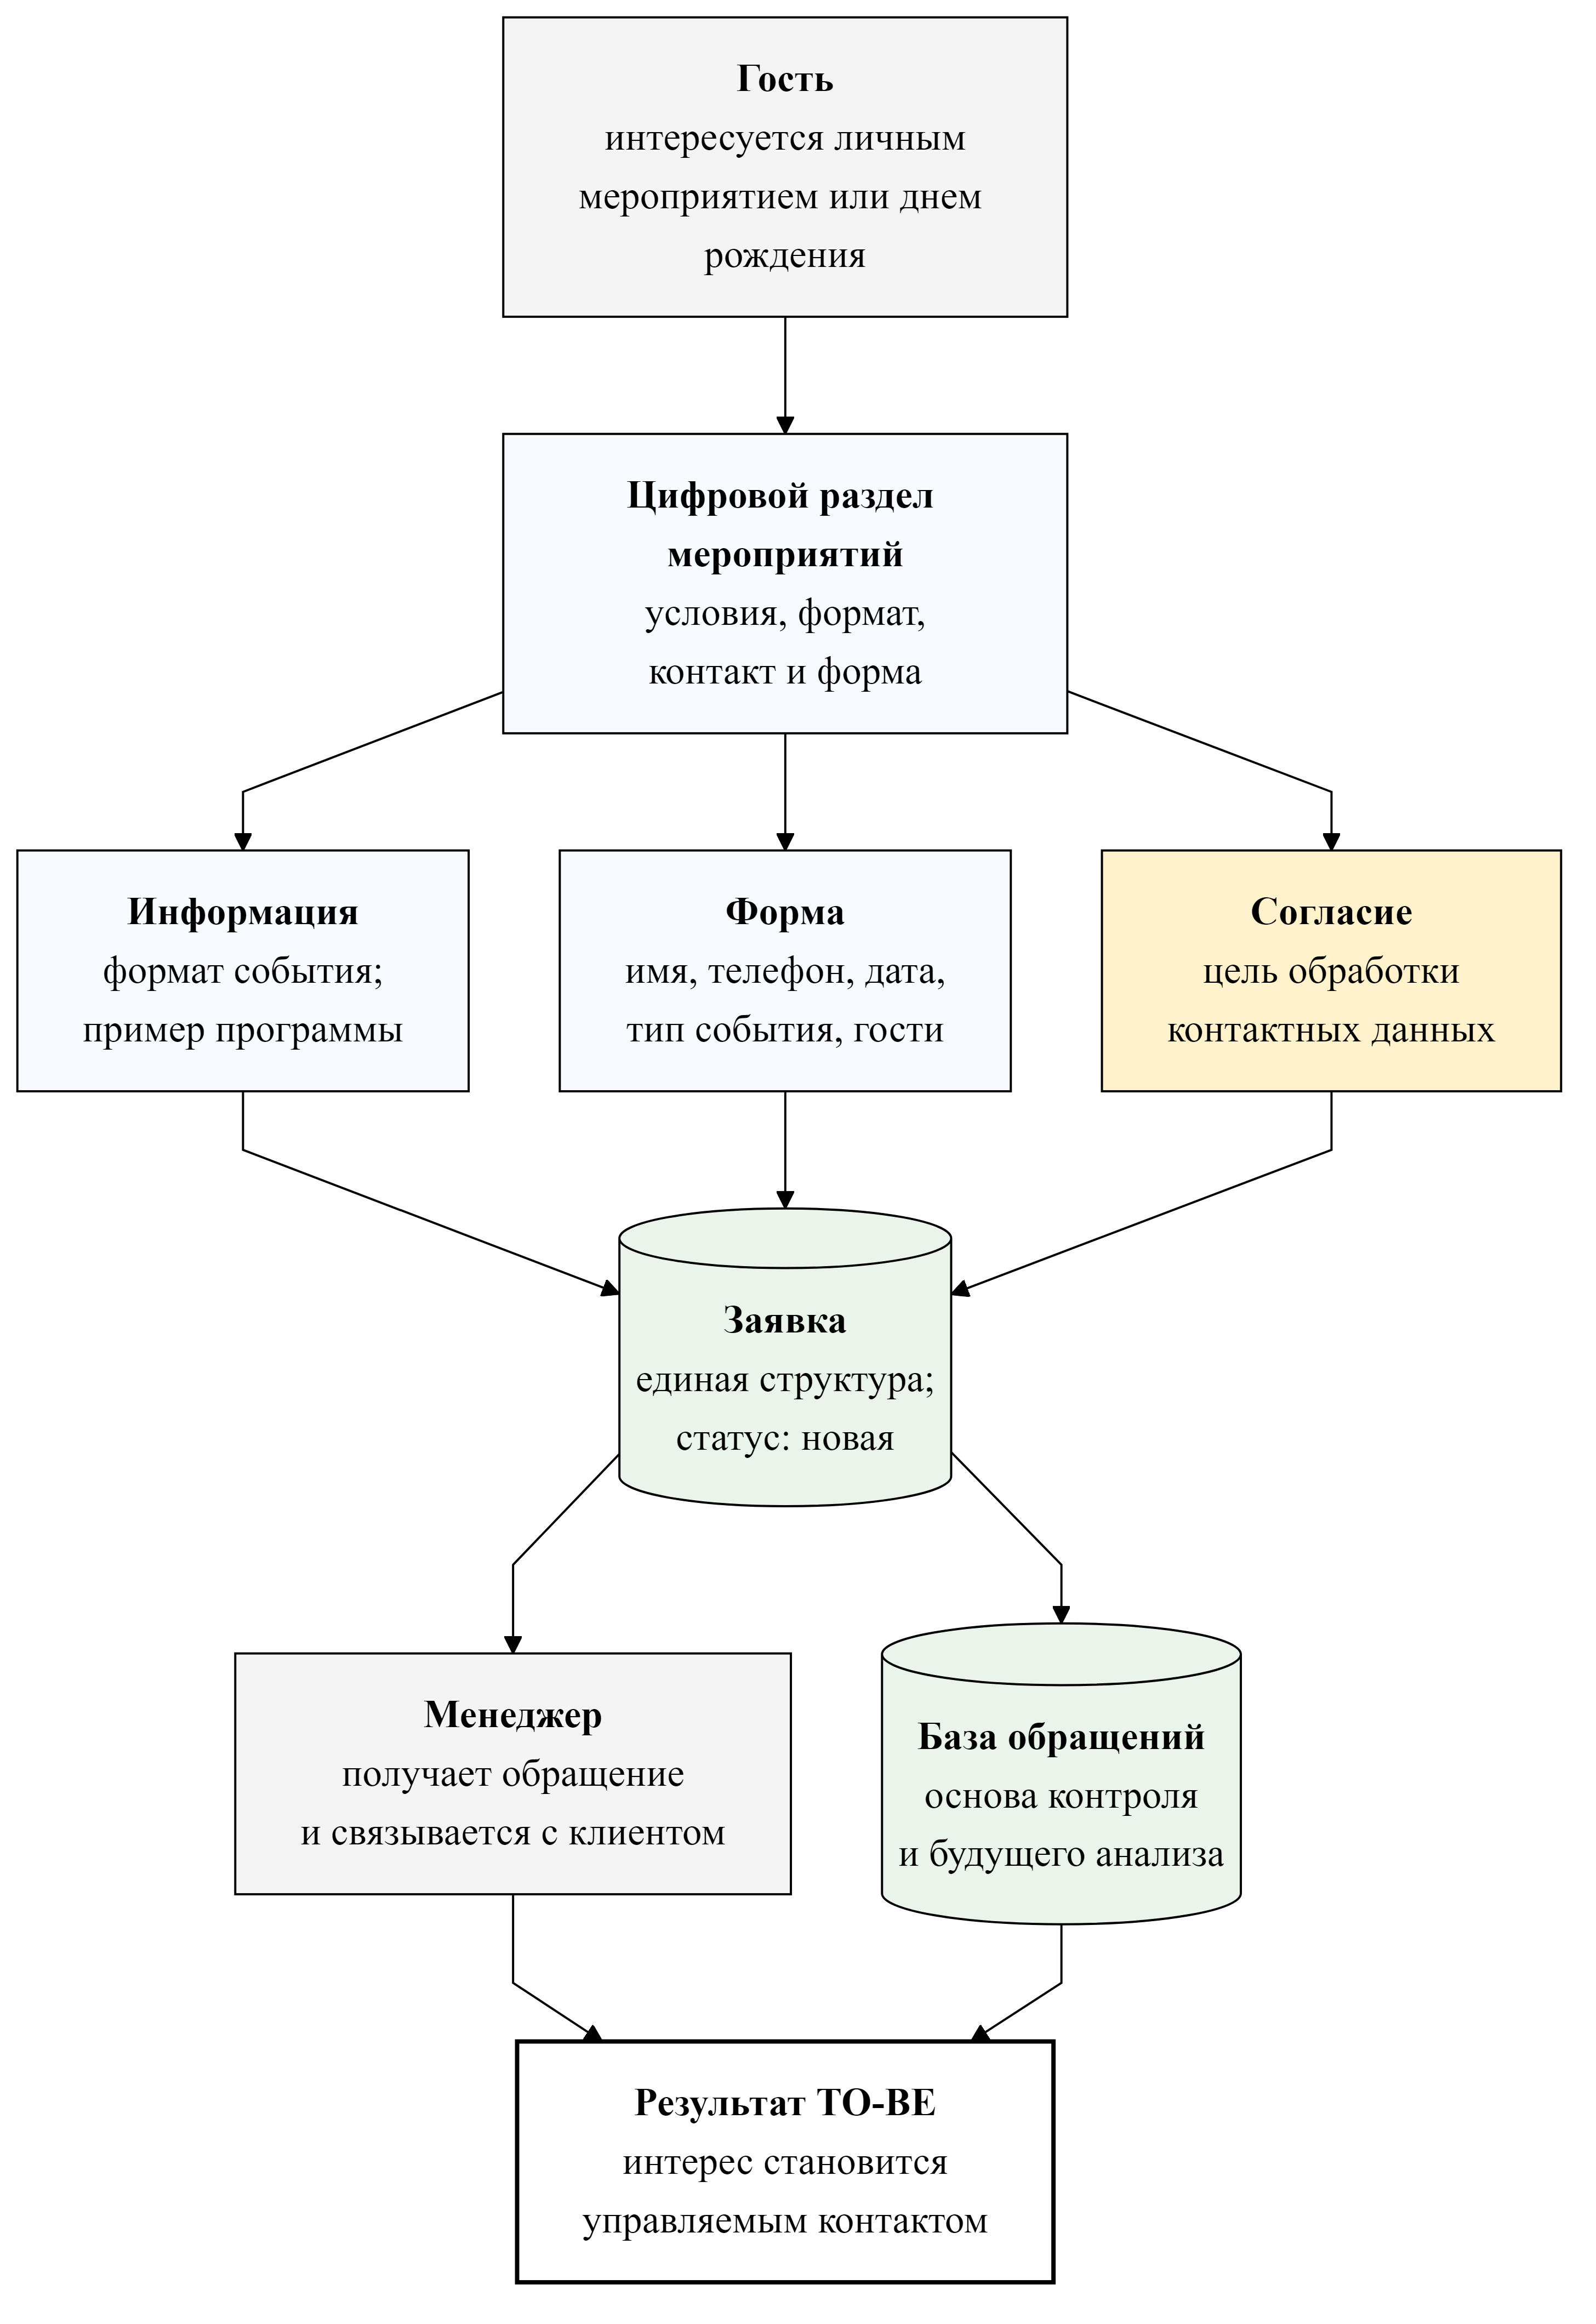
\includegraphics[width=0.98\textwidth,height=0.84\textheight,keepaspectratio]{figures/chapter2_v2_tobe_event_request.png}
    \caption{TO-BE процесс первичной заявки на личное мероприятие}
    \label{fig:v2_tobe_event_request}
\end{figure}

С точки зрения дальнейшего развития TO-BE модель создает основу для накопления данных. Даже если на первом этапе система фиксирует только заявки, просмотры и игровые действия, эти данные могут стать основой для будущих решений: какие события вызывают интерес, какие блюда чаще просматриваются, какие игровые механики возвращают пользователя, какие заявки чаще приводят к контакту менеджера. Литература по аналитике данных подчеркивает, что предиктивные и персонализированные сценарии требуют качественной исходной модели данных и организационной готовности, поэтому их следует рассматривать как развитие, а не как немедленный результат внедрения~\cite{prediktivnaya_crm,ziolkowska2021}.

\section{Геймификация как центральный элемент тематического клиентского опыта}

Геймификация в данной работе должна рассматриваться как центральный проектный элемент, потому что предметная область кафе уже построена вокруг тематического опыта. Если обычное кафе может ограничиться меню, контактами и формой бронирования, то кафе в стилистике Хогвартса создает ожидание участия в воображаемой среде. Следовательно, цифровая система должна не только информировать клиента, но и продолжать тематическую логику заведения в мобильном сценарии.

Научное основание такого подхода задается определением геймификации как использования элементов игрового дизайна в неигровых контекстах~\cite{deterding2011}. Это определение важно для ограничения проектной логики: в работе не проектируется самостоятельная компьютерная игра, конкурирующая с основной услугой кафе. Проектируется клиентский слой, где игровые элементы поддерживают интерес к меню, событиям, мастер-классам, повторному посещению и эмоциональной связи с брендом.

В исследованиях hospitality и tourism геймификация рассматривается как инструмент вовлечения, удовлетворенности, лояльности и повторного взаимодействия, но авторы также предупреждают, что одних очков, уровней и наград недостаточно для устойчивого эффекта~\cite{xu2017,sutrisno2026}. Поэтому проектная геймификация ООО <<\_\_\_\_>> должна быть не механическим начислением баллов, а связанной системой тематических действий. Пользователь должен понимать, зачем он выбирает факультет, открывает заклинания или участвует в уроке, и как это связано с посещением кафе.

В текущем проекте \texttt{webapp} уже заложены элементы, позволяющие сформировать такую систему: факультеты, пользовательский профиль, уровни мастерства, заклинания, уроки, испытания и локально сохраняемый прогресс. Эти элементы можно интерпретировать через три группы мотивации. Факультет и профиль поддерживают идентичность пользователя; уровни, заклинания и прогресс поддерживают ощущение компетентности; уроки, события и возможные командные механики могут поддерживать причастность к тематическому сообществу. Такая логика согласуется с выводами исследований о том, что вовлечение клиента связано не только с утилитарной ценностью, но и с эмоциональными и поведенческими формами участия~\cite{pansari2017,behnam2021,chathoth2016}.

\begin{table}[H]
\centering
\small
\caption{Проектная роль элементов геймификации}
\label{tab:v2_gamification_elements}
\begin{tabularx}{\textwidth}{|>{\raggedright\arraybackslash}p{0.18\textwidth}|>{\raggedright\arraybackslash}p{0.50\textwidth}|>{\raggedright\arraybackslash}X|}
\hline
\textbf{Элемент} & \textbf{Пользовательское действие и проектная функция} & \textbf{Научное основание} \\ \hline
Факультет & Пользователь выбирает принадлежность к тематической группе; система формирует идентичность и персональный вход в цифровой опыт. & Геймификация как gameful design~\cite{deterding2011} \\ \hline
Профиль и уровень & Пользователь видит накопленный прогресс; система поддерживает повторное возвращение и ощущение развития. & Engagement как поведенческое и эмоциональное участие~\cite{pansari2017,behnam2021} \\ \hline
Заклинания & Пользователь открывает новые тематические действия; цифровой прогресс связывается с атмосферой кафе. & Gamification in tourism and hospitality~\cite{xu2017,sutrisno2026} \\ \hline
Уроки и испытания & Пользователь проходит короткие сценарии внутри webapp; взаимодействие становится запоминающимся до или после визита. & Co-creation and customer engagement~\cite{chathoth2016} \\ \hline
Кубок факультетов & Действия пользователя могут суммироваться в общий результат; появляется основа для социального и событийного вовлечения. & Роль социальных affordances в геймифицированных платформах~\cite{buil2024} \\ \hline
\end{tabularx}
\normalsize
\end{table}

Из таблицы~\ref{tab:v2_gamification_elements} следует, что геймификация должна быть связана с реальными клиентскими сценариями. Если пользователь только нажимает на игровые элементы, но не получает связи с меню, событиями или посещением кафе, проектный эффект будет слабым. Поэтому в TO-BE модели игровые действия должны постепенно связываться с содержанием кафе: тематические задания могут вести к знакомству с разделами меню, события могут становиться поводом для открытия нового урока, а повторное посещение webapp может поддерживаться новым сезонным контентом.

\begin{figure}[p]
    \centering
    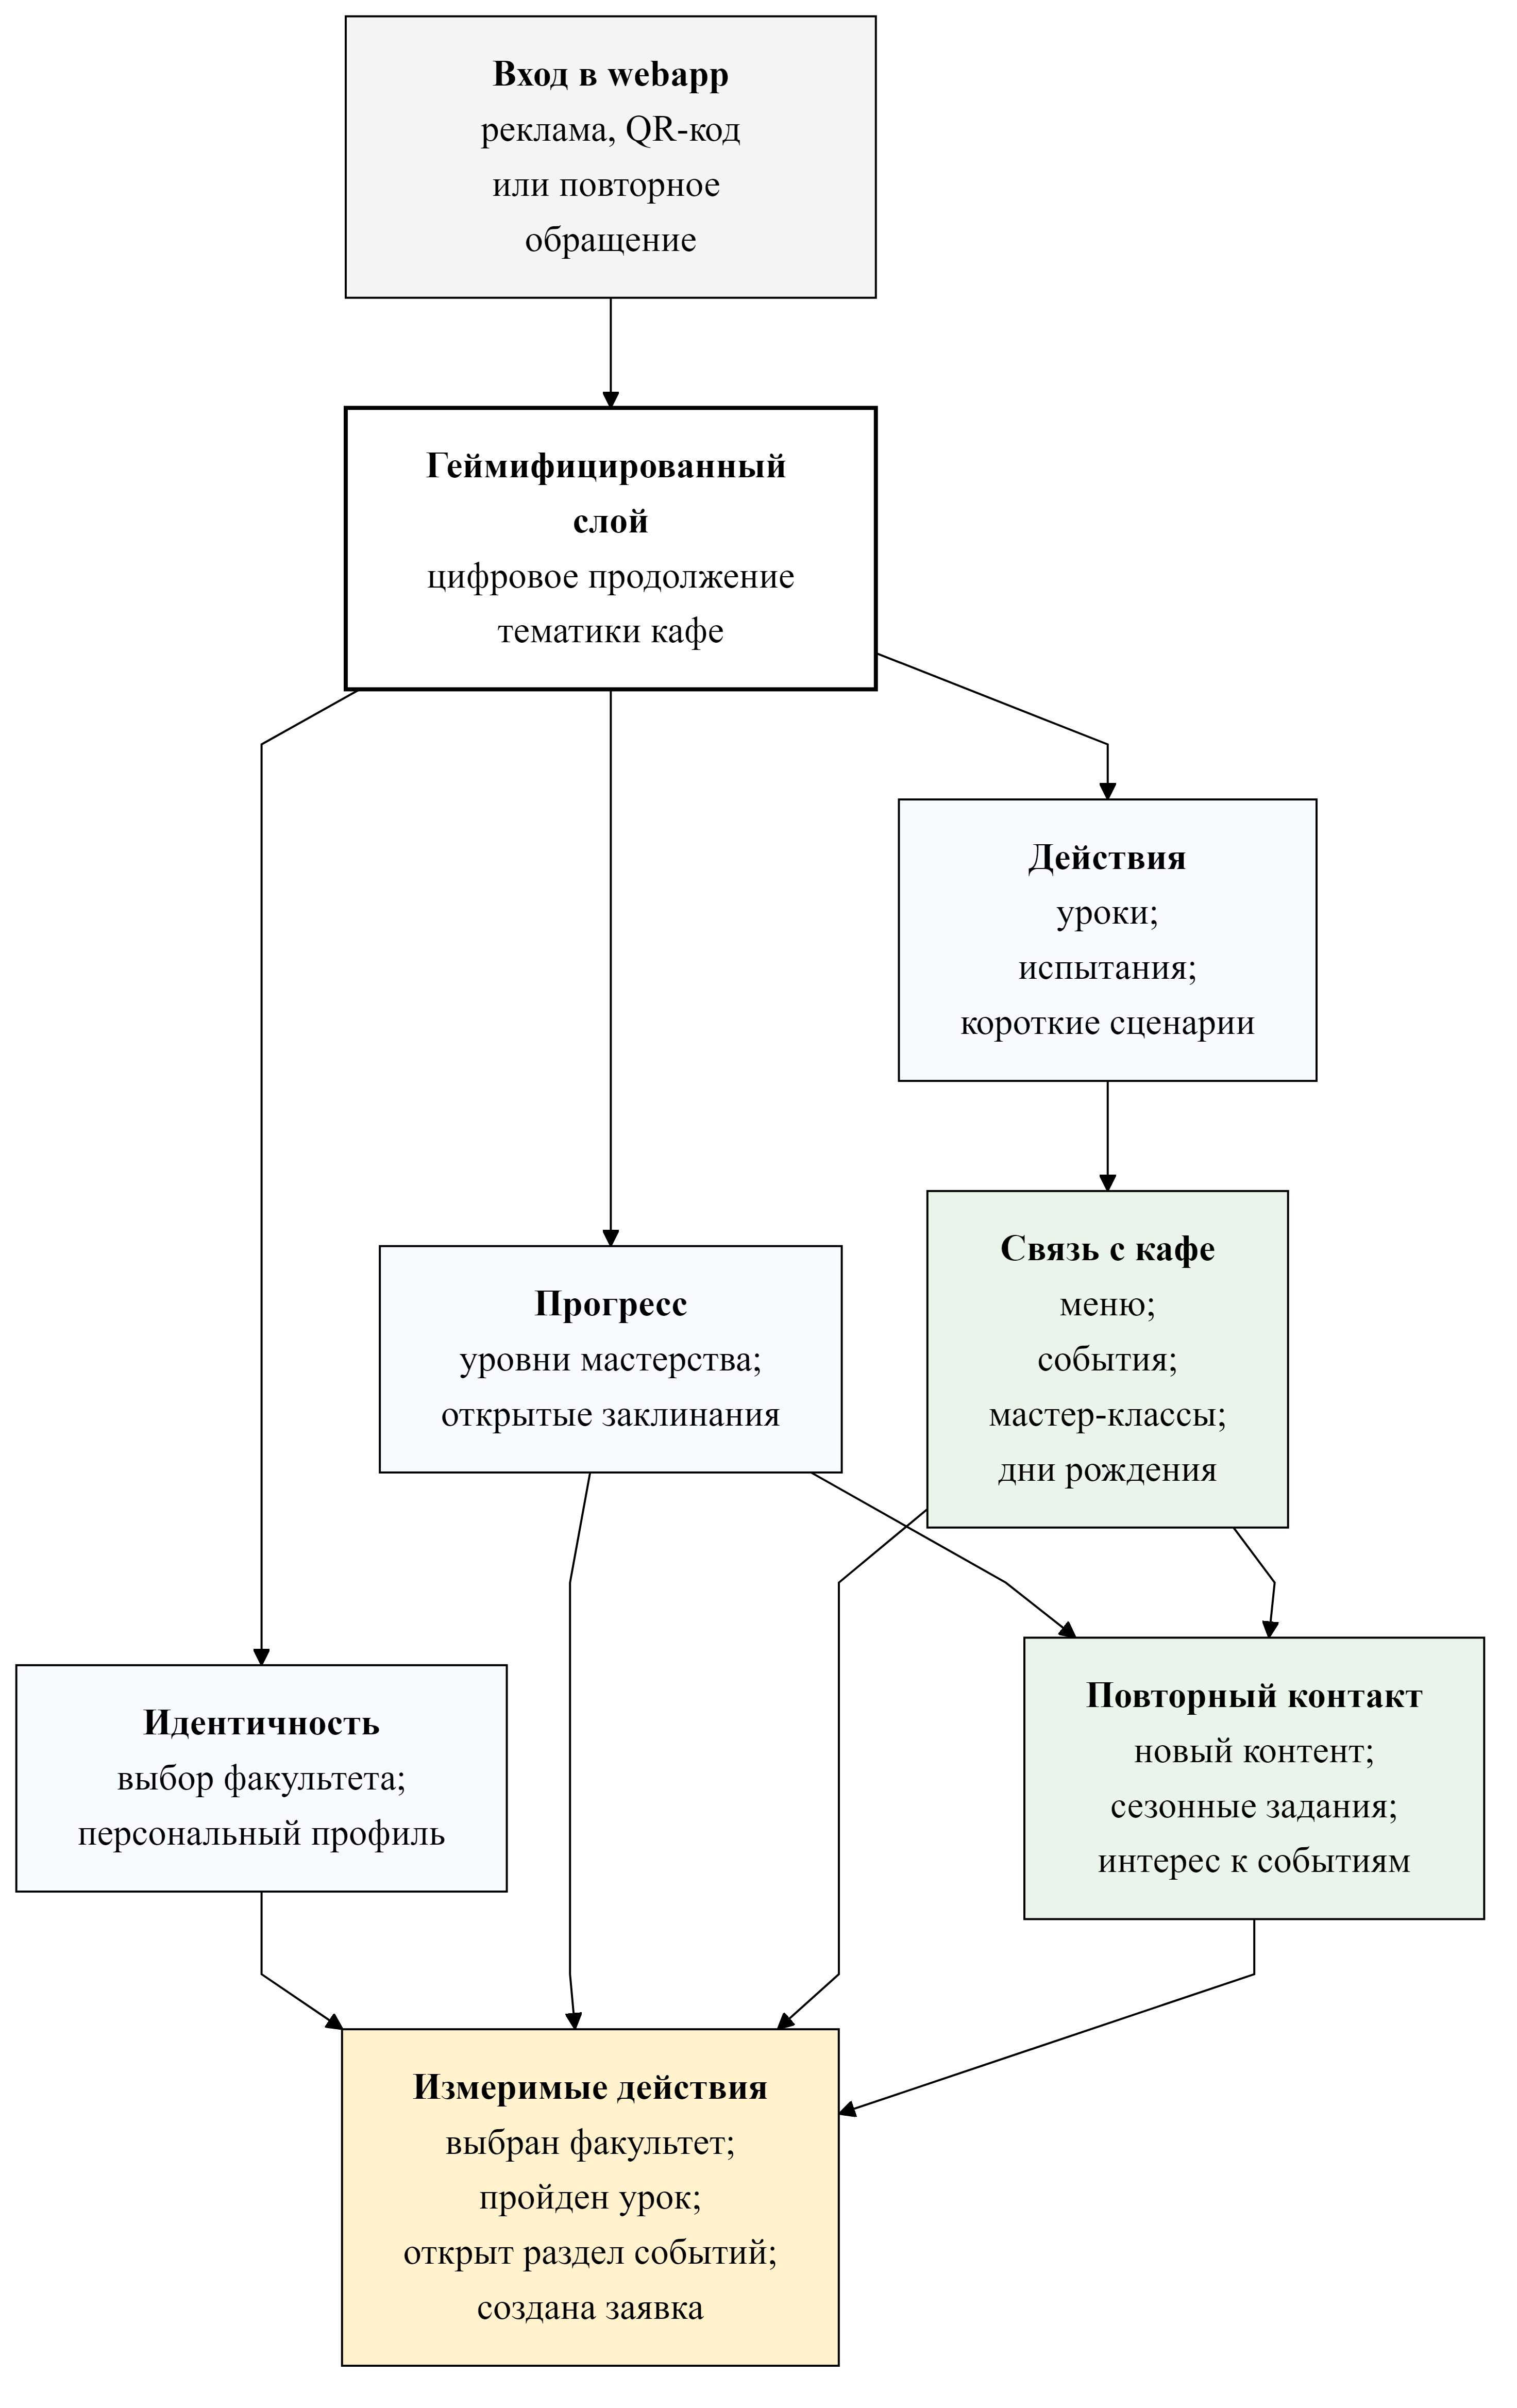
\includegraphics[width=0.98\textwidth,height=0.84\textheight,keepaspectratio]{figures/chapter2_v2_gamification_journey.png}
    \caption{Пользовательский путь в геймифицированном слое webapp}
    \label{fig:v2_gamification_journey}
\end{figure}

Такой подход позволяет корректно сформулировать ожидаемый эффект. Нельзя заранее утверждать, что геймификация гарантированно увеличит выручку или удержание, поскольку для этого нужны данные после внедрения. Однако можно обоснованно утверждать, что геймифицированный слой создает дополнительные точки взаимодействия с клиентом, расширяет клиентский опыт за пределы утилитарного поиска информации и формирует измеримые цифровые действия. Для молодой организации это особенно полезно, потому что такие действия могут стать ранними индикаторами интереса к бренду, событиям и повторному посещению.

\section{Требования к информационной системе и трассируемость}

Требования к системе выводятся из AS-IS ограничений, TO-BE модели и фактических ролей пользователей. Такой порядок важен, потому что требования без трассируемости превращаются в список функций, не связанный с исследуемой проблемой. В работах по pre-requirements traceability подчеркивается, что полезно связывать требования с источниками их возникновения, заинтересованными сторонами и причинами изменения~\cite{mucha2024}. Поэтому в данной работе каждое ключевое требование должно иметь основание в факте обследования, научном источнике или правовом ограничении.

Функциональные требования должны покрывать минимальный клиентский контур. Гость должен просматривать меню, события и информацию о личных мероприятиях; отправлять заявку; нажимать на телефон менеджера; взаимодействовать с геймифицированным сценарием. Менеджер должен получать структурированные сведения заявки и понимать ее статус. Управляющая должна иметь возможность обновлять контент, поскольку без этого цифровой канал быстро потеряет актуальность. Такая структура требований соответствует определению автоматизированной системы как совокупности функций, данных, пользователей и организационного применения~\cite{gost34003,utkin_baldin_2003}.

Нефункциональные требования должны учитывать мобильный характер сценария. Пользователь, пришедший из рекламы или QR-кода, не должен проходить длинный путь до меню, телефона или формы заявки. Исследования PWA подчеркивают, что такой формат объединяет свойства веба и приложения, но требует внимания к совместимости, доступности, безопасности и качеству мобильного интерфейса~\cite{fauzan2022,pwa_implementation_2024}. Поэтому качество интерфейса следует оценивать через понятность, быстрый доступ к ключевым действиям, устойчивость на мобильных устройствах и минимизацию лишнего ввода.

\begin{table}[H]
\centering
\footnotesize
\caption{Функциональные требования к клиентскому цифровому контуру}
\label{tab:v2_functional_requirements}
\setlength{\tabcolsep}{4pt}
\begin{tabularx}{\textwidth}{|>{\raggedright\arraybackslash}p{0.10\textwidth}|>{\raggedright\arraybackslash}p{0.64\textwidth}|>{\raggedright\arraybackslash}X|}
\hline
\textbf{ID} & \textbf{Требование и основание} & \textbf{Роли} \\ \hline
FR-01 & Предоставлять единый клиентский интерфейс для сведений о кафе, меню, событиях, контактах и личных мероприятиях. \newline \textbf{Основание:} отсутствие собственного цифрового канала. & Гость \\ \hline
FR-02 & Отображать актуальные категории меню и карточки блюд с описанием, ценой и статусом доступности. \newline \textbf{Основание:} неполная информация о меню до визита. & Гость, управляющая \\ \hline
FR-03 & Отображать события, мастер-классы и форматы личных мероприятий с понятными условиями участия. \newline \textbf{Основание:} планируемая событийная модель кафе. & Гость, управляющая \\ \hline
FR-04 & Позволять гостю отправлять первичную заявку на мероприятие или день рождения с минимально необходимыми контактными данными. \newline \textbf{Основание:} неочевидный канал обращения к менеджеру. & Гость, менеджер \\ \hline
FR-05 & Передавать заявку менеджеру в структурированном виде и сохранять ее статус как объект дальнейшей обработки. \newline \textbf{Основание:} ручная фиксация договоренностей у менеджера. & Менеджер \\ \hline
FR-06 & Предоставлять возможность прямого звонка менеджеру из раздела мероприятий и контактного блока. \newline \textbf{Основание:} требование управляющей о возможности позвонить менеджеру. & Гость, менеджер \\ \hline
FR-07 & Поддерживать выбор факультета, профиль, прогресс, уроки и игровые действия в геймифицированном слое. \newline \textbf{Основание:} тематический формат кафе и реализуемая клиентская часть. & Гость \\ \hline
FR-08 & Фиксировать согласие на обработку персональных данных перед отправкой формы заявки. \newline \textbf{Основание:} наличие имени, телефона и иных контактных сведений в форме. & Гость, менеджер \\ \hline
FR-09 & Допускать обновление меню, событий и тематического контента без изменения клиентского интерфейса. \newline \textbf{Основание:} потребность в управляемом цифровом канале. & Управляющая, администратор \\ \hline
FR-10 & Формировать основу для последующего анализа заявок, просмотров событий и геймифицированных действий. \newline \textbf{Основание:} необходимость будущей оценки клиентского интереса. & Управляющая, владелец \\ \hline
\end{tabularx}
\normalsize
\end{table}

\begin{table}[H]
\centering
\small
\caption{Нефункциональные требования к клиентскому цифровому контуру}
\label{tab:v2_nonfunctional_requirements}
\begin{tabularx}{\textwidth}{|>{\raggedright\arraybackslash}p{0.13\textwidth}|>{\raggedright\arraybackslash}p{0.48\textwidth}|>{\raggedright\arraybackslash}X|}
\hline
\textbf{ID} & \textbf{Требование} & \textbf{Критерий приемки} \\ \hline
NFR-01 & Клиентский интерфейс должен быть приспособлен к мобильному сценарию доступа из рекламы, QR-кода или повторного обращения & Меню, события, телефон и форма заявки доступны с мобильного экрана без перехода во внешние каналы \\ \hline
NFR-02 & Навигация должна снижать неопределенность пользователя по сравнению с AS-IS состоянием & Пользователь может самостоятельно найти меню, события, адрес, телефон и условия личного мероприятия \\ \hline
NFR-03 & Формы должны минимизировать состав обязательных персональных данных относительно цели конкретного сценария & Обязательными остаются только данные, необходимые для связи менеджера с клиентом \\ \hline
NFR-04 & Система должна отделять публичные клиентские функции от будущих административных функций & Гость не имеет доступа к управлению контентом, заявками и клиентскими данными \\ \hline
NFR-05 & Архитектура должна допускать поэтапное развитие от клиентской части к серверной обработке заявок и административному интерфейсу & Новые серверные компоненты добавляются без переписывания клиентского webapp \\ \hline
NFR-06 & Геймификация не должна блокировать основные коммерческие сценарии & Из игрового раздела пользователь может вернуться к меню, событиям, контактам или заявке \\ \hline
NFR-07 & Интерфейс должен сохранять тематическую согласованность без перегрузки текста и лишнего ввода & Игровые элементы связаны с концепцией кафе и не увеличивают путь к ключевым действиям \\ \hline
NFR-08 & Система должна поддерживать совместимость с современными мобильными и настольными браузерами & Клиентские сценарии доступны через браузер без обязательной установки отдельного приложения \\ \hline
\end{tabularx}
\normalsize
\end{table}

\begin{table}[H]
\centering
\small
\caption{Трассируемость проблем, требований и проектных решений}
\label{tab:v2_requirements_traceability}
\begin{tabularx}{\textwidth}{|>{\raggedright\arraybackslash}p{0.23\textwidth}|>{\raggedright\arraybackslash}p{0.48\textwidth}|>{\raggedright\arraybackslash}X|}
\hline
\textbf{Проблема AS-IS} & \textbf{Требование и проектное решение} & \textbf{Критерий проверки} \\ \hline
Нет единого источника информации & Пользователь должен получить меню, события, контакты и описание мероприятий в одном интерфейсе. \newline \textbf{Решение:} публичная клиентская часть webapp. & Пользователь находит основные сведения без обращения к менеджеру \\ \hline
Неочевидный канал заявки & Пользователь должен иметь понятную форму первичного обращения. \newline \textbf{Решение:} форма заявки на личное мероприятие. & Заявка содержит обязательные поля и может быть передана менеджеру \\ \hline
Ручная фиксация контактов & Система должна нормировать состав данных обращения. \newline \textbf{Решение:} сущность заявки с полями контакта, даты, типа события и комментария. & Все заявки имеют одинаковую структуру данных \\ \hline
Тематический опыт не поддержан цифровым образом & Пользователь должен иметь игровые действия, связанные с концепцией кафе. \newline \textbf{Решение:} факультеты, профиль, уровни, заклинания, уроки. & Пользователь может начать и продолжить игровой прогресс \\ \hline
Персональные данные собираются через форму & Система должна ограничить цель и состав обработки данных. \newline \textbf{Решение:} согласие, политика обработки и минимальный набор полей. & До отправки формы пользователь видит основание обработки данных \\ \hline
\end{tabularx}
\normalsize
\end{table}

Таблица~\ref{tab:v2_requirements_traceability} задает минимальную проверяемую рамку требований. В дальнейшем она может быть расширена административными сценариями, аналитикой и интеграциями, но для текущей ВКР важно сохранить соответствие фактической готовности проекта. Клиентская часть и геймификация уже являются сильной реализуемой частью, тогда как серверные и административные компоненты должны описываться как проектируемые или развиваемые, если к моменту защиты они не будут полностью завершены.

\section{Информационное обеспечение и данные}

Информационное обеспечение проектируемой системы должно описывать не только таблицы базы данных, но и смысл данных в клиентском процессе. В классической логике информационных систем данные становятся управленческим ресурсом только тогда, когда они имеют структуру, источник возникновения, цель обработки и связь с функциями системы~\cite{utkin_baldin_2003,gost34003}. Поэтому модель данных должна выводиться из клиентского пути, а не из абстрактного желания создать базу.

Первый блок данных связан с публичным контентом: меню, категории блюд, карточки блюд, события, мастер-классы, описание личных мероприятий и контактные сведения. Эти данные не являются персональными, но от их актуальности зависит качество pre-visit этапа. Второй блок связан с заявками: имя, телефон, дата, тип мероприятия, количество гостей, комментарий и статус обработки. Третий блок связан с геймификацией: профиль пользователя, выбранный факультет, уровень, открытые элементы и история действий. Четвертый блок связан с правовыми основаниями: согласие, цель обработки, дата и версия текста согласия~\cite{fz152,moric2024}.

\begin{table}[H]
\centering
\small
\caption{Основные группы данных проектируемой системы}
\label{tab:v2_data_groups}
\begin{tabularx}{\textwidth}{|>{\raggedright\arraybackslash}p{0.22\textwidth}|>{\raggedright\arraybackslash}p{0.48\textwidth}|>{\raggedright\arraybackslash}X|}
\hline
\textbf{Группа данных} & \textbf{Примеры атрибутов и источник} & \textbf{Назначение} \\ \hline
Контент кафе & Название блюда, категория, описание, цена, событие, время проведения. \newline \textbf{Источник:} управляющая или администратор. & Информирование клиента до визита и внутри кафе \\ \hline
Заявка на мероприятие & Имя, телефон, дата, тип события, число гостей, комментарий, статус. \newline \textbf{Источник:} клиентская форма. & Первичный контакт и последующая обработка менеджером \\ \hline
Профиль и игровой прогресс & Факультет, уровень, открытые заклинания, пройденные уроки. \newline \textbf{Источник:} действия пользователя в webapp. & Поддержка геймифицированного опыта и повторного взаимодействия \\ \hline
Согласие и правовые сведения & Текст согласия, дата, цель обработки, версия документа. \newline \textbf{Источник:} интерфейс формы и настройки системы. & Подтверждение правомерности обработки персональных данных \\ \hline
Обратная связь и реакции & Оценка, текст отзыва, связь с событием или посещением. \newline \textbf{Источник:} пользовательский сценарий после визита или события. & Основа для анализа клиентского опыта и улучшения сервиса \\ \hline
\end{tabularx}
\normalsize
\end{table}

Для текущего этапа проекта важно разделить данные, которые уже могут существовать в клиентской реализации, и данные, которые должны появиться при подключении серверной части. Элементы локального игрового профиля могут храниться в браузере пользователя, что подходит для раннего прототипа и демонстрации клиентского опыта. Однако заявки на мероприятия и согласия на обработку персональных данных не должны оставаться только локальным состоянием клиента, потому что их назначение состоит в передаче менеджеру и последующей организационной обработке.

\begin{table}[H]
\centering
\footnotesize
\caption{Персональные данные, цели обработки и проектные меры}
\label{tab:v2_personal_data_purposes}
\setlength{\tabcolsep}{4pt}
\begin{tabularx}{\textwidth}{|>{\raggedright\arraybackslash}p{0.21\textwidth}|>{\raggedright\arraybackslash}p{0.46\textwidth}|>{\raggedright\arraybackslash}X|}
\hline
\textbf{Группа данных} & \textbf{Примеры полей и цель обработки} & \textbf{Проектная мера} \\ \hline
Контактные данные заявки & Имя, телефон, комментарий клиента. \newline \textbf{Цель:} связь менеджера с потенциальным клиентом по вопросу личного мероприятия или дня рождения. & Минимизация обязательных полей, явная цель обработки, согласие до отправки формы \\ \hline
Параметры мероприятия & Дата, тип события, количество гостей, пожелания. \newline \textbf{Цель:} первичная оценка возможности проведения мероприятия и подготовка обратного звонка. & Статус заявки, дата создания, ограниченный доступ менеджера \\ \hline
Геймифицированный профиль & Факультет, уровень, открытые элементы, прогресс. \newline \textbf{Цель:} поддержка тематического цифрового опыта и повторного взаимодействия. & Разделение локального игрового состояния и персональных контактных данных \\ \hline
Согласия & Цель обработки, версия текста, дата принятия. \newline \textbf{Цель:} подтверждение правового основания обработки персональных данных. & Отдельная фиксация факта согласия и версии текста \\ \hline
Будущие административные действия & Исполнитель, операция, объект, время, результат. \newline \textbf{Цель:} контроль операций с заявками, контентом и согласиями. & Журналирование действий, влияющих на клиентские данные и статусы \\ \hline
\end{tabularx}
\normalsize
\end{table}

Минимальная инфологическая модель должна включать сущности меню, блюда, события, заявки, клиентского контакта, согласия, игрового профиля и игрового действия. Связь между заявкой и клиентским контактом позволяет менеджеру обработать обращение; связь между согласием и заявкой фиксирует правовое основание; связь между игровым профилем и игровыми действиями позволяет анализировать участие пользователя без немедленного построения сложной CRM. Такой набор сущностей достаточен для первой версии клиентского цифрового контура и не подменяет собой полную ERP-автоматизацию кафе.

\begin{figure}[p]
    \centering
    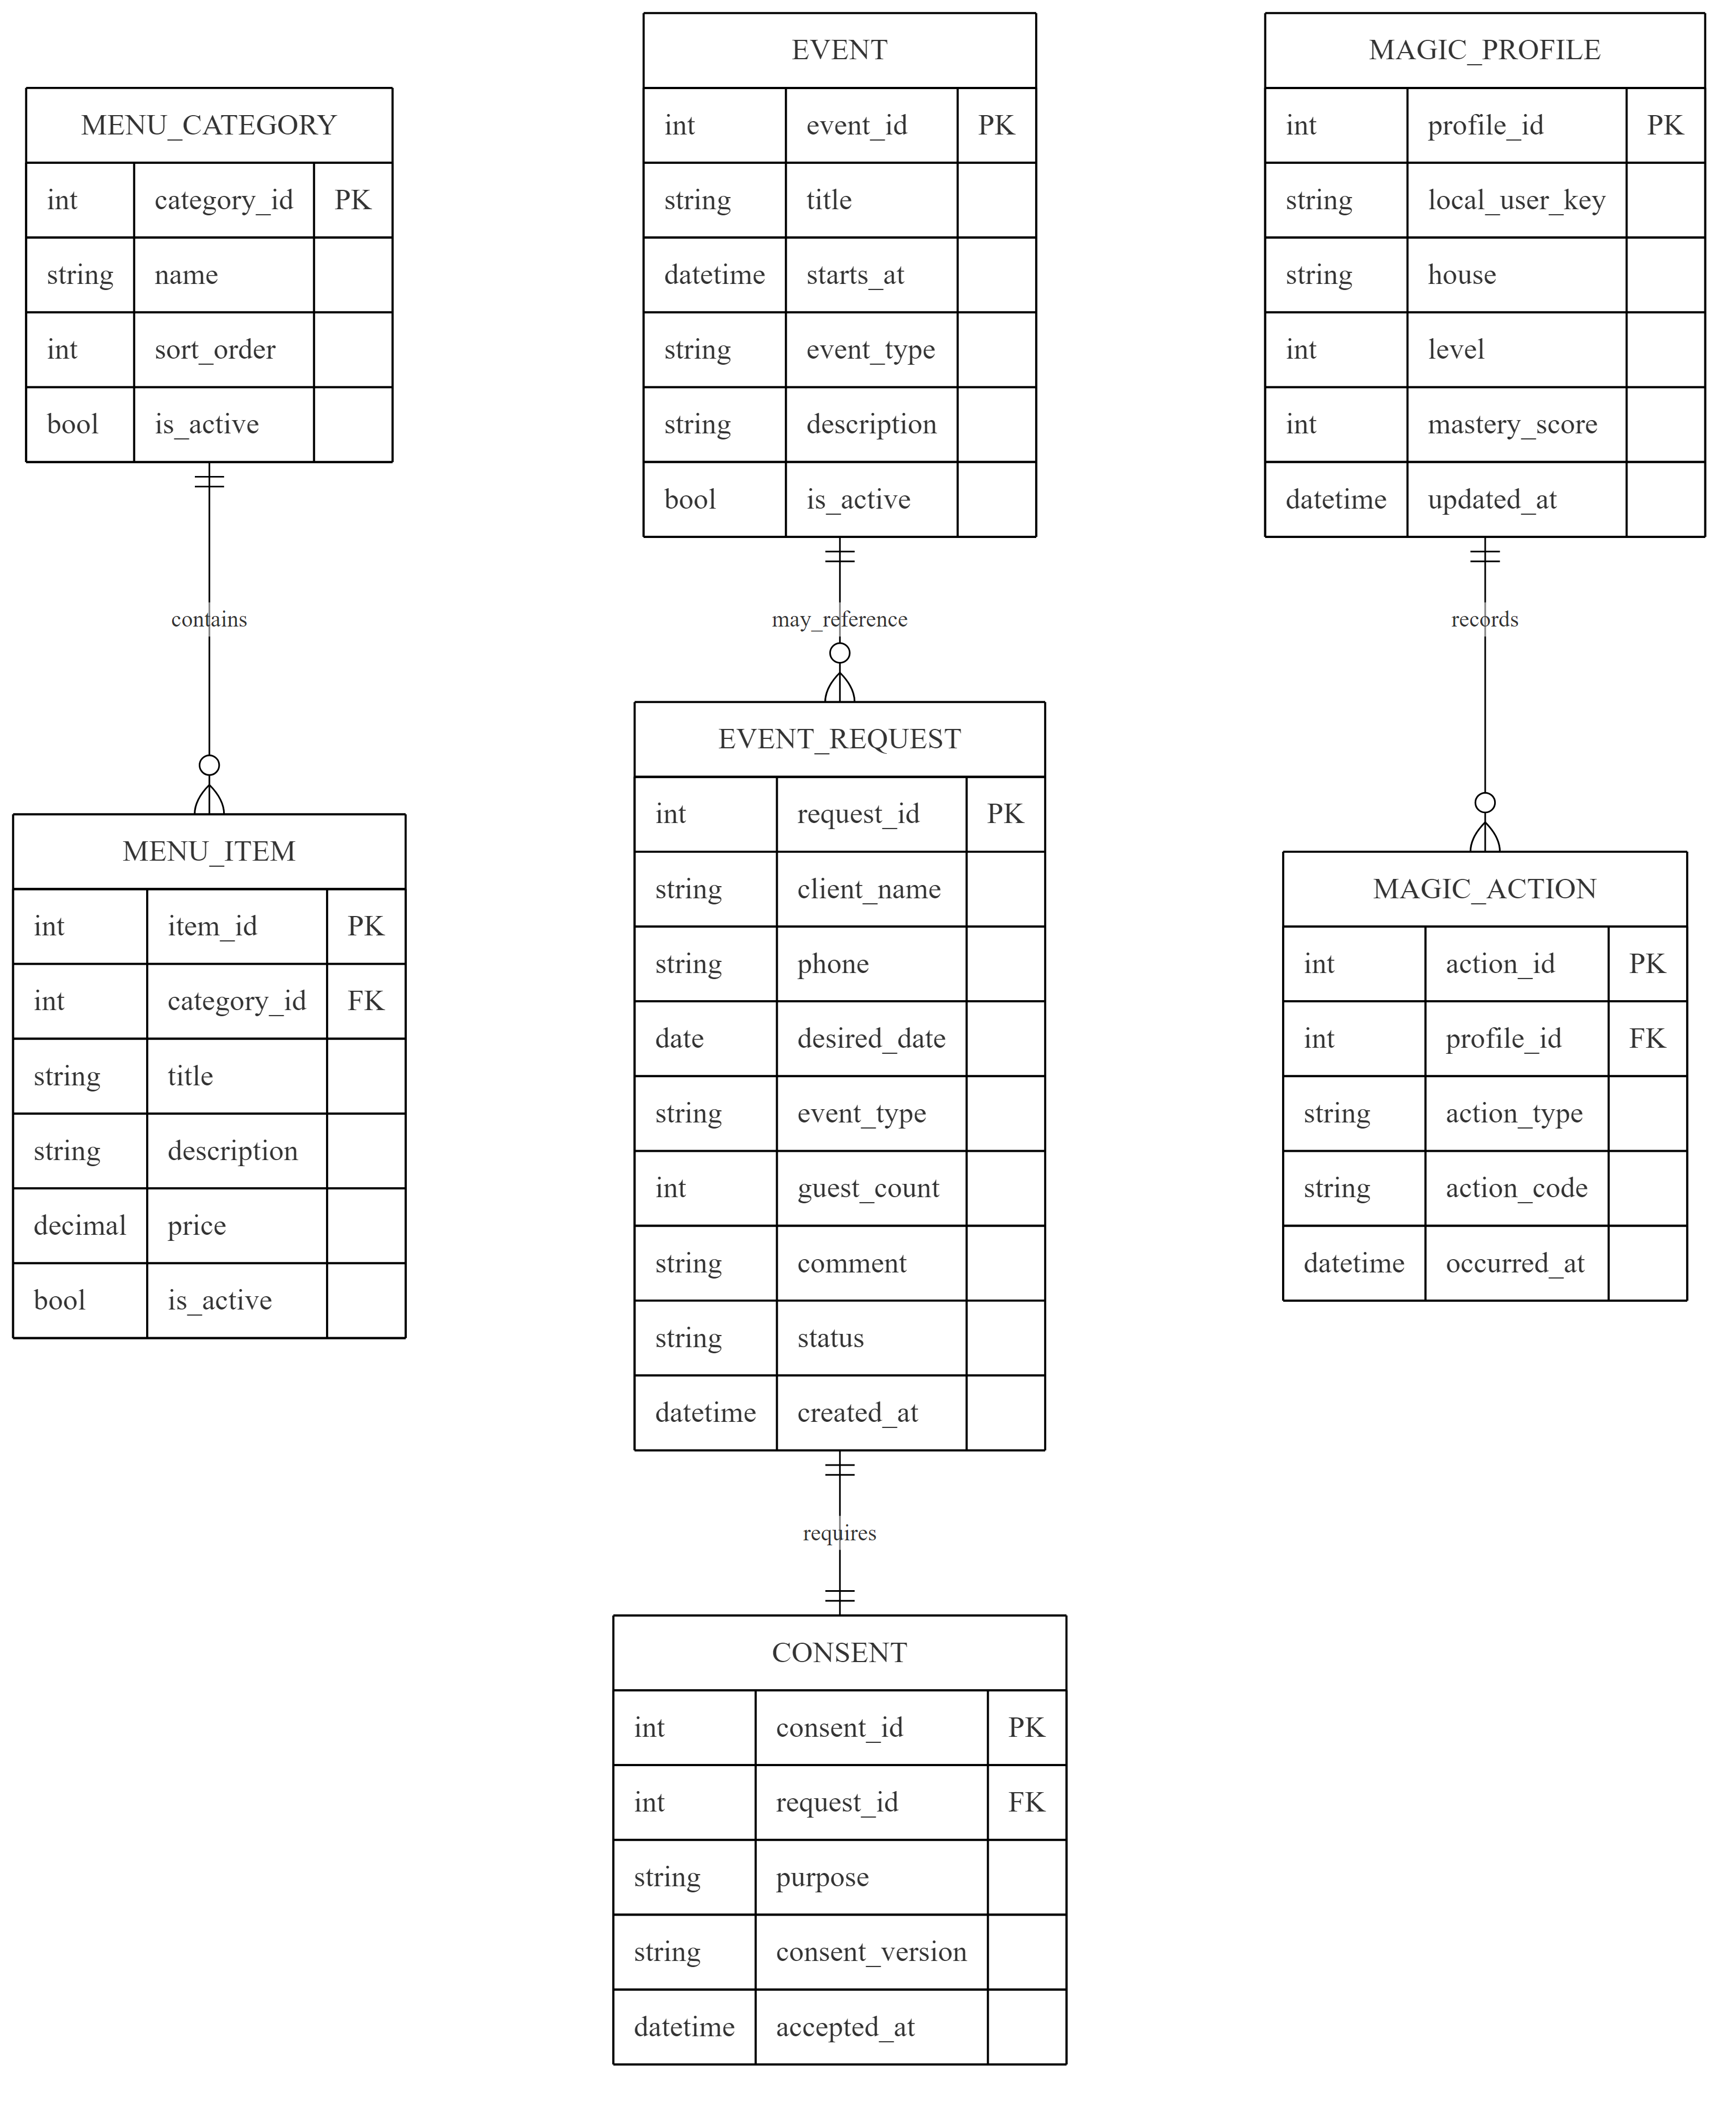
\includegraphics[width=0.98\textwidth,height=0.84\textheight,keepaspectratio]{figures/chapter2_v2_data_model.png}
    \caption{Концептуальная модель данных клиентского цифрового контура}
    \label{fig:v2_data_model}
\end{figure}

\section{Архитектура и технологический способ реализации}

Архитектурное решение должно соответствовать двум условиям: мобильному клиентскому сценарию и поэтапной готовности проекта. Анализ текущей папки \texttt{webapp} показывает, что клиентская часть реализуется на React и Vite, а пользовательский интерфейс включает разделы главной страницы, меню, событий, игры и дополнительной информации. Такой выбор соответствует задаче быстрого мобильного доступа, поскольку клиент может открыть сервис из браузера, рекламной ссылки или QR-кода без обязательной установки нативного приложения.

С точки зрения архитектуры программного обеспечения важно разделить пользовательский интерфейс, данные, бизнес-логику и внешние точки интеграции. В литературе по архитектуре ПО такое разделение рассматривается как способ управлять изменениями, качественными атрибутами и дальнейшей эволюцией системы~\cite{bass2021,iso25010_2023}. Для рассматриваемого проекта это означает, что клиентская часть должна быть отделена от будущего API заявок, административного интерфейса и хранилища данных.

PWA-подход является обоснованным для данной задачи, потому что кафе нуждается в мобильном канале с низким барьером входа. Исследования PWA показывают, что такие приложения объединяют свойства веба и мобильных приложений: они доступны через браузер, могут устанавливаться на устройство и поддерживать отдельные сценарии работы при нестабильном соединении~\cite{fauzan2022,pwa_implementation_2024}. При этом PWA не следует описывать как универсальное решение всех проблем, поскольку его ограничения связаны с браузерной поддержкой, безопасностью, доступностью и особенностями мобильного интерфейса~\cite{fauzan2022}.

\begin{table}[H]
\centering
\small
\caption{Архитектурные компоненты клиентского цифрового контура}
\label{tab:v2_architecture_components}
\begin{tabularx}{\textwidth}{|>{\raggedright\arraybackslash}p{0.23\textwidth}|>{\raggedright\arraybackslash}p{0.33\textwidth}|>{\raggedright\arraybackslash}X|}
\hline
\textbf{Компонент} & \textbf{Назначение} & \textbf{Статус в проектной логике} \\ \hline
Клиентское web/PWA-приложение & Отображение меню, событий, контактов, заявок и геймификации & Реализуемое ядро текущей работы \\ \hline
Модуль контента & Хранение и публикация сведений о меню, событиях и мероприятиях & Проектируемый слой данных и управления \\ \hline
Модуль заявок & Прием и передача первичных обращений менеджеру & Ключевой серверный сценарий для дальнейшей реализации \\ \hline
Модуль согласий & Фиксация цели и факта согласия на обработку персональных данных & Обязательный правовой слой для форм с контактными данными \\ \hline
Геймификационный модуль & Профиль, факультет, прогресс, уроки и игровые действия & Отличительный клиентский слой, уже частично представленный в webapp \\ \hline
Административный интерфейс & Обновление контента и обработка заявок сотрудниками & Направление развития после стабилизации клиентской части \\ \hline
\end{tabularx}
\normalsize
\end{table}

Таблица~\ref{tab:v2_architecture_components} фиксирует поэтапность реализации. Клиентская часть и геймификация могут быть продемонстрированы как готовое ядро, тогда как серверная обработка заявок, административное управление и аналитика могут развиваться итерационно. Такая архитектурная честность важна для ВКР, потому что текст должен отражать фактическую готовность проекта и не выдавать будущие функции за уже внедренные.

\begin{figure}[p]
    \centering
    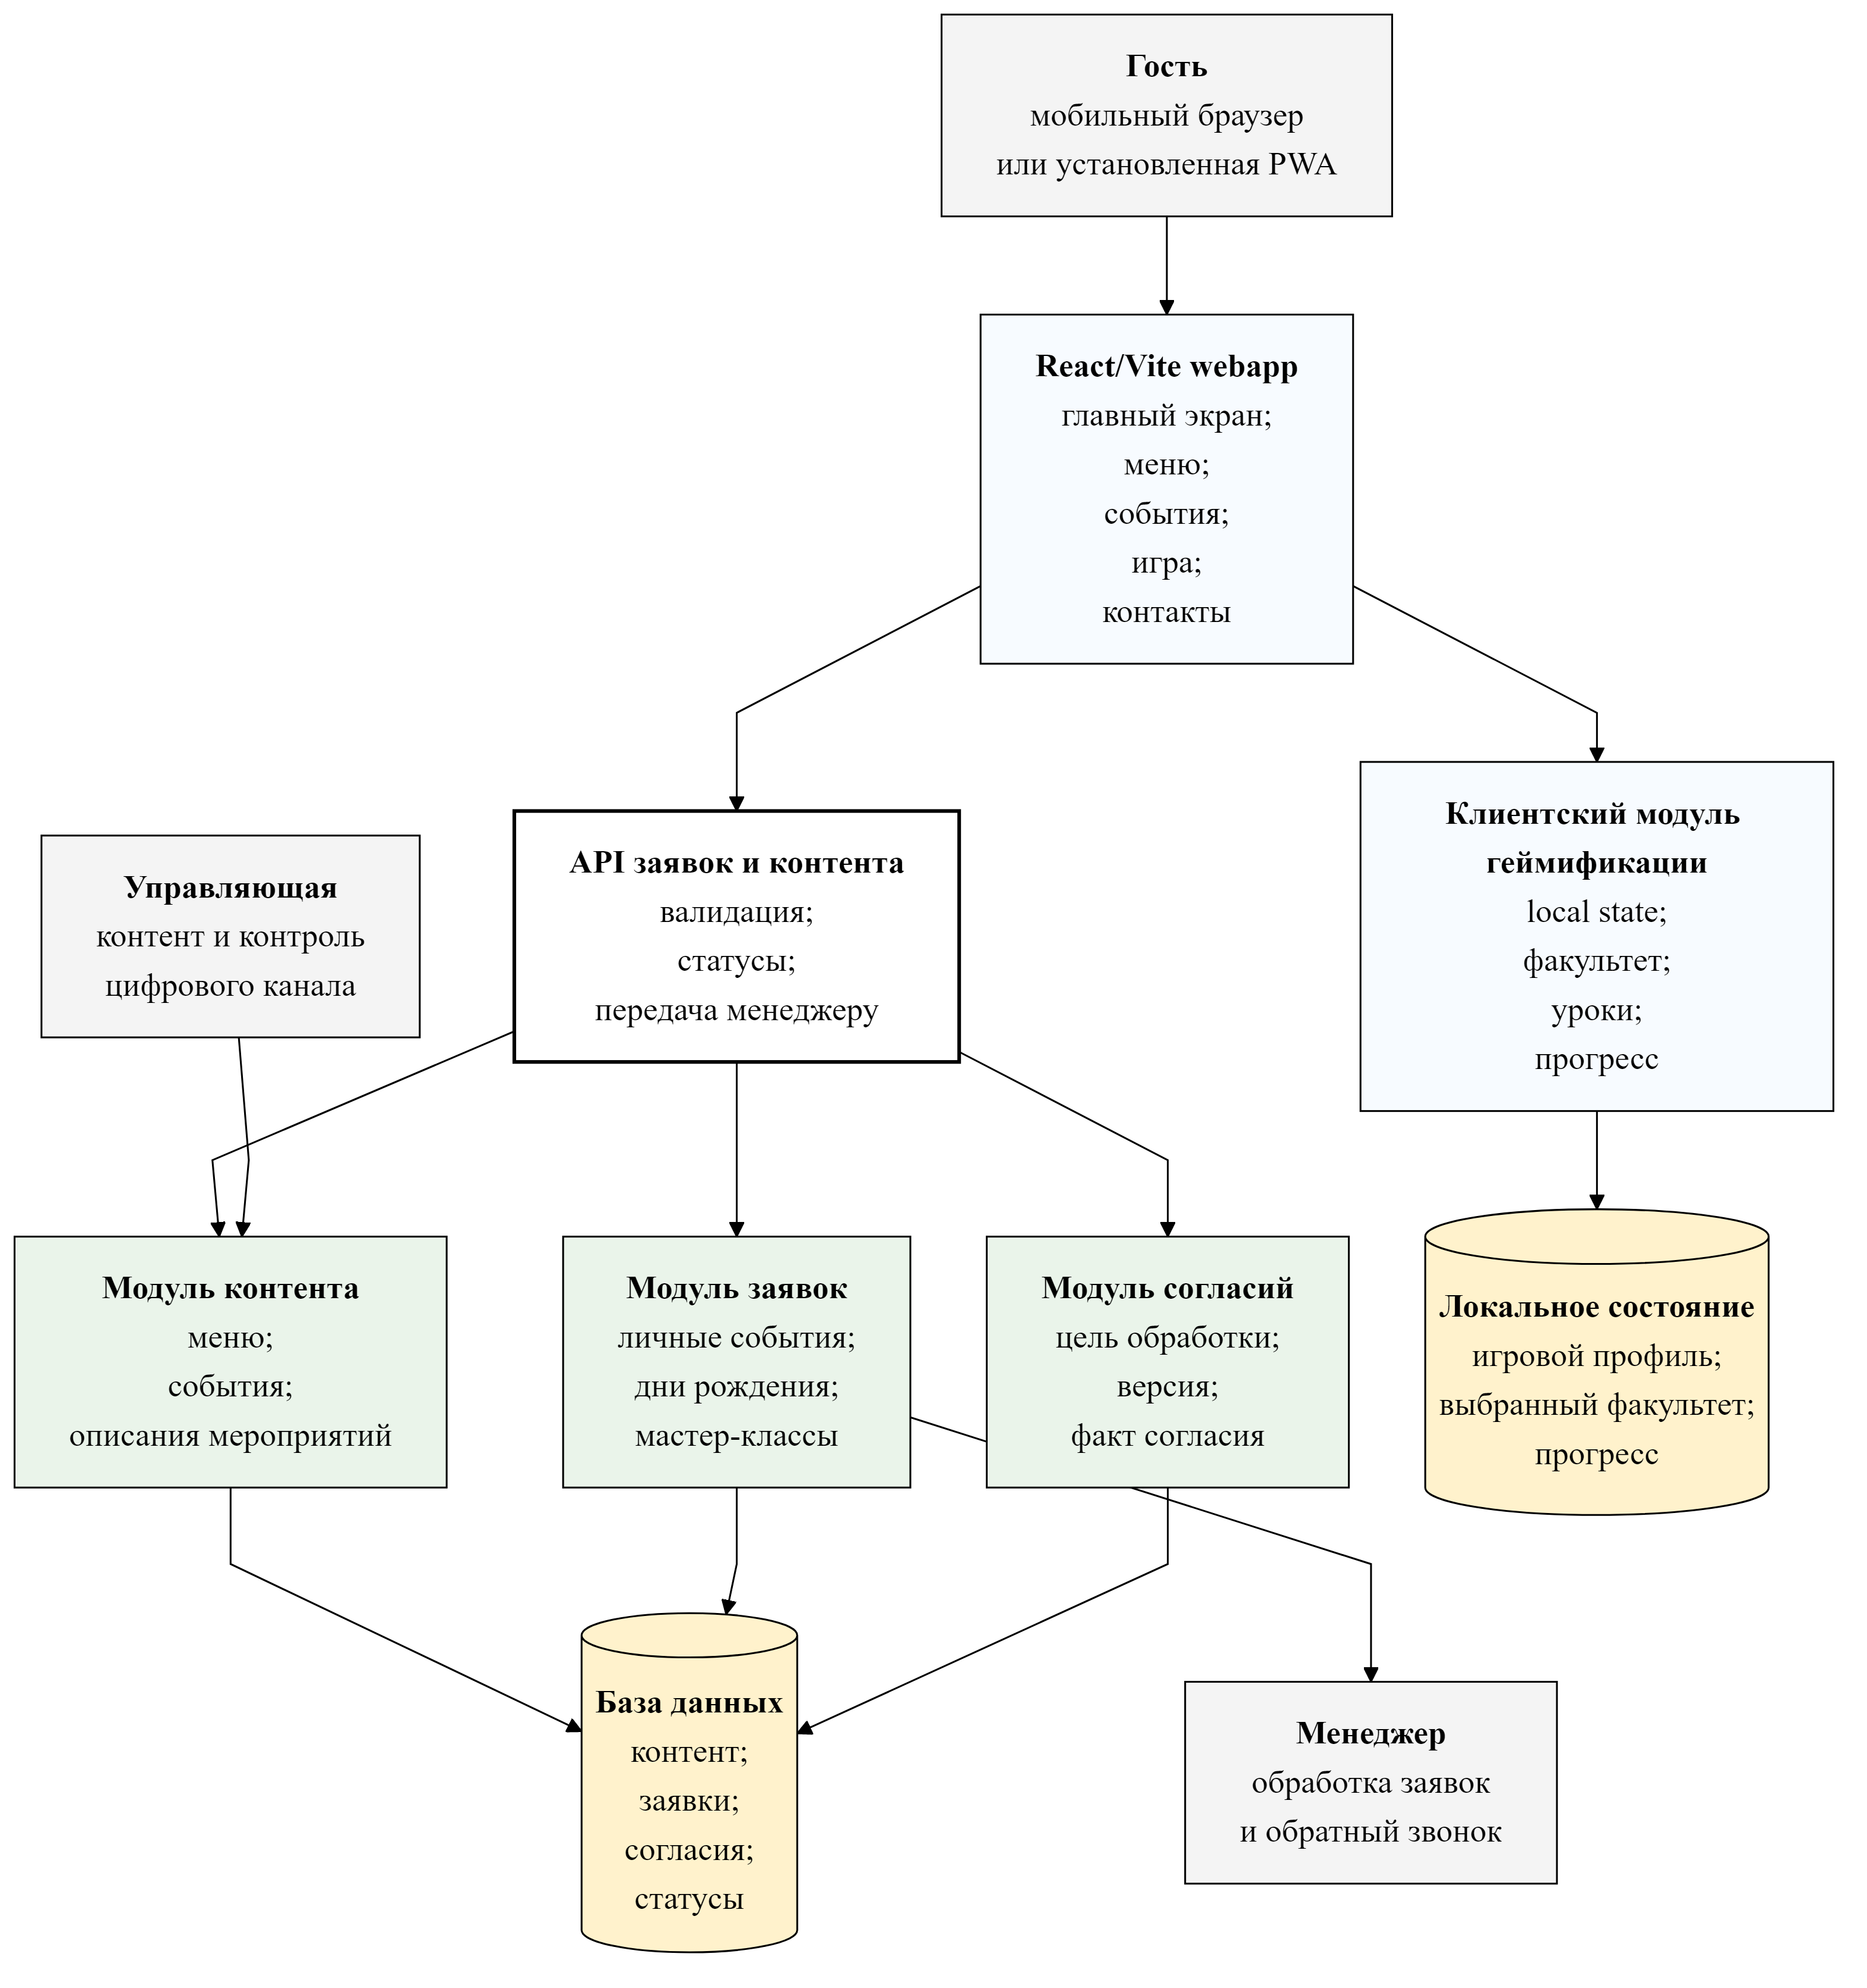
\includegraphics[width=0.98\textwidth,height=0.84\textheight,keepaspectratio]{figures/chapter2_v2_architecture.png}
    \caption{Архитектура клиентского цифрового контура с поэтапным развитием серверных компонентов}
    \label{fig:v2_architecture}
\end{figure}

\section{Пользовательские сценарии и критерии проверки}

Пользовательские сценарии нужны для проверки того, что требования действительно превращаются в действия пользователя. В user experience подходе качество интерфейса оценивается относительно конкретных пользователей, целей и контекста использования~\cite{norman2013,iso25010_2023}. Поэтому для ООО <<\_\_\_\_>> следует проверять не абстрактную красоту интерфейса, а способность гостя быстро решить практическую задачу: посмотреть меню, найти событие, отправить заявку или продолжить тематический опыт.

Первый сценарий, знакомство с кафе до визита, начинается с перехода из рекламы, поиска или QR-кода. Пользователь должен увидеть концепцию кафе, меню, события, адрес и возможность связи. Критерий проверки состоит в том, что клиент может получить базовую информацию без звонка менеджеру и без физического посещения. Этот сценарий закрывает главный AS-IS разрыв pre-visit этапа.

Второй сценарий, заявка на личное мероприятие, начинается с интереса к дню рождения или частному событию. Пользователь должен открыть раздел мероприятий, понять формат услуги, заполнить короткую форму и увидеть, что менеджер свяжется с ним для уточнения деталей. Критерий проверки состоит в наличии всех обязательных полей, понятной цели передачи данных и возможности прямого звонка менеджеру.

Третий сценарий, участие в тематическом цифровом опыте, начинается с выбора факультета или открытия игрового раздела. Пользователь должен совершить понятное действие, увидеть прогресс и получить мотив продолжить взаимодействие. Критерий проверки состоит не в немедленной покупке, а в наличии измеримого цифрового действия: выбран факультет, открыт уровень, пройден урок, выполнено задание или пользователь вернулся в игровой раздел.

\begin{table}[H]
\centering
\small
\caption{Пользовательские сценарии и критерии проверки}
\label{tab:v2_user_scenarios}
\begin{tabularx}{\textwidth}{|>{\raggedright\arraybackslash}p{0.20\textwidth}|>{\raggedright\arraybackslash}p{0.50\textwidth}|>{\raggedright\arraybackslash}X|}
\hline
\textbf{Сценарий} & \textbf{Действия пользователя и ожидаемый результат} & \textbf{Критерий проверки} \\ \hline
Знакомство до визита & Пользователь открывает webapp, смотрит меню, события, адрес и контакты; клиент понимает, что предлагает кафе и как с ним связаться. & Основные сведения доступны за короткий путь в интерфейсе \\ \hline
Заявка на мероприятие & Пользователь открывает раздел личного события, заполняет форму и подтверждает отправку; менеджер получает структурированное обращение. & Все обязательные поля заполнены, цель обработки данных указана \\ \hline
Звонок менеджеру & Пользователь нажимает на телефон или кнопку связи; интерфейс переводит его к прямому контакту. & Сценарий доступен из раздела мероприятий и контактного блока \\ \hline
Геймификация & Пользователь выбирает факультет, открывает урок и видит прогресс; webapp формирует тематический цифровой опыт. & Прогресс сохраняется и отображается в интерфейсе \\ \hline
Возврат к событиям & Пользователь повторно открывает расписание или игровой раздел; система поддерживает повторное взаимодействие. & Есть обновляемый контент и понятный маршрут к новым действиям \\ \hline
\end{tabularx}
\normalsize
\end{table}

\begin{table}[H]
\centering
\small
\caption{Связь экранов интерфейса с пользовательскими задачами, требованиями и данными}
\label{tab:v2_screens_requirements_data}
\begin{tabularx}{\textwidth}{|>{\raggedright\arraybackslash}p{0.19\textwidth}|>{\raggedright\arraybackslash}p{0.43\textwidth}|>{\raggedright\arraybackslash}X|}
\hline
\textbf{Экран} & \textbf{Пользовательская задача и требования} & \textbf{Данные} \\ \hline
Главный экран & Получить единую точку входа в клиентский цифровой контур. \newline \textbf{Требования:} FR-01; NFR-01. & Ссылки на меню, события, контакт, мероприятия и игровой раздел \\ \hline
Меню и карточка блюда & Найти блюдо, описание, цену и актуальность позиции. \newline \textbf{Требование:} FR-02. & Категория, блюдо, описание, цена, статус доступности \\ \hline
События и мастер-классы & Выбрать мероприятие и понять условия участия. \newline \textbf{Требование:} FR-03. & Событие, дата, формат, описание, доступность \\ \hline
Личное мероприятие & Понять формат дня рождения или частного события и оставить заявку. \newline \textbf{Требования:} FR-04, FR-05, FR-06, FR-08. & Контакт, дата, тип мероприятия, число гостей, комментарий, согласие \\ \hline
Игровой раздел & Выбрать факультет, пройти урок и увидеть прогресс. \newline \textbf{Требования:} FR-07; NFR-06, NFR-07. & Факультет, уровень, открытые элементы, игровые действия \\ \hline
Контакты & Быстро перейти к звонку менеджеру или уточнить адрес. \newline \textbf{Требования:} FR-01, FR-06. & Телефон, адрес, часы работы, маршрут обращения \\ \hline
Будущая административная часть & Обновлять контент и обрабатывать заявки. \newline \textbf{Требования:} FR-05, FR-09, FR-10. & Контент, заявки, статусы, согласия, журнал действий \\ \hline
\end{tabularx}
\normalsize
\end{table}

Проверка сценариев должна быть связана с этапом готовности проекта. Для клиентской части можно использовать экспертный просмотр, мобильную проверку интерфейса и ручное прохождение сценариев. Для серверной части после реализации нужно добавить проверку передачи данных, хранения заявок, фиксации согласий и прав доступа. Для геймификации важно отдельно проверить, что игровые элементы не закрывают основные коммерческие действия, а поддерживают их: пользователь должен легко вернуться из игрового раздела к меню, событиям или форме заявки.

\section{Выводы по второй главе}

Во второй главе объект исследования был рассмотрен как действующее тематическое кафе на раннем этапе запуска. Анализ показал, что основная проблема AS-IS состояния состоит не в большом объеме необработанных заявок, а в отсутствии собственного управляемого цифрового канала, который связывает рекламный интерес, информацию о меню и событиях, заявку на личное мероприятие и дальнейший контакт менеджера.

На основании AS-IS анализа была сформирована TO-BE модель клиентского цифрового контура. В нее включены публичная клиентская часть, цифровое меню, раздел событий, форма заявки на личное мероприятие, возможность звонка менеджеру, минимальная правовая логика обработки персональных данных и геймифицированный слой. Такая модель соответствует фактическому состоянию кафе и не подменяет проект полной ERP-автоматизацией.

Особое место в проектной модели занимает геймификация. Для тематического кафе она является не декоративным дополнением, а способом продлить атмосферу заведения в цифровой среде, сформировать дополнительные точки взаимодействия и подготовить базу для будущего анализа клиентского вовлечения. При этом ожидаемый эффект сформулирован осторожно: геймификация создает условия для интереса, повторного контакта и измеримых цифровых действий, но ее экономический результат должен подтверждаться после внедрения.

Сформированные требования, группы данных, архитектурные компоненты и пользовательские сценарии задают основу для последующей реализации. Ключевой принцип дальнейшей работы состоит в трассируемости: каждая функция должна быть связана с проблемой AS-IS состояния, ролью пользователя, научным основанием или правовым ограничением. Такой подход позволяет сохранить научную выводимость текста и сделать вторую главу не описанием интерфейса, а полноценной аналитико-проектной частью ВКР.
